\chapter{Electric circuits}\fancyfoot[LO,RE]{Physics: Electricity and Magnetism}

\section{Potential difference and emf}

When a circuit is connected and complete, charge can move through the circuit. Charge will not move unless there is a reason, a force to drive it round the circuit. Think of it as though charge is at rest and something has to push it along. This means that work needs to be done to make charge move. A force acts on the charges, doing work, to make them move. The force is provided by the battery in the circuit.

A battery has the potential to drive charge round a closed circuit, the battery has potential energy that can be converted into electrical energy by doing work on the charge in the circuit to make it move. 

\subsection*{Voltmeter}
\begin{minipage}{.5\textwidth}
A voltmeter is an instrument for measuring the work done to drive charge between two
points in an electric circuit which we call the potential difference because the work done is 
the different in the potential energy.

The symbol for a voltmeter is:
\begin{center}
\begin{pspicture}(-2,0)(3,3)
%\psgrid
\pnode(0,0){A} \pnode(0,3){B} \pnode(3,3){C} \pnode(3,0){D}
%\battery(A)(B){}
\circledipole[parallel,parallelnode,parallelsep=.5,labeloffset=0](A)(B){V}
%\psline(B)(C) \resistor[dipolestyle=rectangle](C)(D){} \psline(D)(A)
\end{pspicture}
% \caption{A voltmeter should be connected in parallel in a
% circuit.} \label{fig:p:em:ec10:voltmeter}
\end{center}
\end{minipage}
\begin{minipage}{.5\textwidth}
\begin{center}
A voltmeter\\
\includegraphics[width=.8\textwidth]{photos/volts_windy__Flickr.jpg}\\
\textit{Photography by windy\_ on Flickr.}
\end{center}
\end{minipage}

\subsection*{EMF}
\begin{minipage}{.5\textwidth}
When you measure the potential difference across (or between) the terminals of a battery you are measuring the ``electromotive force'' (emf) of the battery. This is the maximum amount of work the battery can do to drive charge from one terminal, through the circuit, to the other terminal.
\end{minipage}
\begin{minipage}{.5\textwidth}
\begin{center}
\begin{pspicture}(-2,0)(3,3)
%\psgrid
\pnode(0,0){A} \pnode(0,3){B} \pnode(3,3){C} \pnode(3,0){D}
\battery(A)(B){}
\circledipole[parallel,parallelnode,parallelsep=.5,labeloffset=0](A)(B){V}
%\psline(B)(C) \resistor[dipolestyle=rectangle](C)(D){} \psline(D)(A)
\end{pspicture}
% \caption{A voltmeter should be connected in parallel in a
% circuit.} \label{fig:p:em:ec10:voltmeter}
\end{center}
\end{minipage}

% This driving potential energy is equal to the total potential energy used in the circuit. This means that the voltage across the battery is equal to the sum of the voltages in the circuit.
% 
% We can use this information to solve problems in which the voltages across elements in a circuit add up to the emf. 
% \begin{equation*}
% EMF = V_{total}
% \end{equation*}
% 
% 
% We call the moving charge "current" and we will talk about this later. The amount of work to move a charge from one point to another point is called potential difference. 

% The position of the charge in the circuit tells you how much potential energy it has because of the force being exerted on it. This is like the force from gravity, the higher an object is above the ground (position) the more potential energy it has.
% 

% Notice that it is a difference between the value of potential energy at two points so we say that potential difference is measured between or across two points. We do not say potential difference through something.


\Definition{Potential Difference}{Potential difference is the difference in electrical potential energy per unit charge between two points. The units of potential difference are the volt (V) which is defined as one joule per coulomb.\\
Symbol: V\hspace{2cm} Unit: V\hspace{2cm} S.I. Units: $\text{J} \cdot \text{C}^{-1}$}

\IFact{The volt is named after the Italian physicist Alessandro Volta (1745--1827).} 

Electrical potential difference is also called voltage.

\begin{minipage}{.5\textwidth}
When you measure the potential difference across (or between) the terminals of a battery that is \textbf{in a complete circuit} you are measuring the terminal potential difference of the battery. Although this is measured in volts it is not identical to the emf. The difference will be the work done to drive charge through the battery.
\end{minipage}
\begin{minipage}{.5\textwidth}
\begin{center}
\begin{pspicture}(-2,0)(3,3)
%\psgrid
\pnode(0,0){A} \pnode(0,3){B} \pnode(3,3){C} \pnode(3,0){D}
\battery(A)(B){}
\circledipole[parallel,parallelnode,parallelsep=.5,labeloffset=0](A)(B){V}
\psline(B)(C) \resistor[dipolestyle=rectangle](C)(D){} \psline(D)(A)
\end{pspicture}
% \caption{A voltmeter should be connected in parallel in a
% circuit.} \label{fig:p:em:ec10:voltmeter}
\end{center}
\end{minipage}
\begin{minipage}{.5\textwidth}
\begin{center}
Batteries\\
\includegraphics[width=.8\textwidth]{photos/batterystack.jpg}\\
\textit{Photography on Flickr.}
\end{center} 
\end{minipage}
\begin{minipage}{.5\textwidth}
One lead of the voltmeter is connected
to one end of the battery and the other lead is connected to the
opposite end. The voltmeter may also be used to measure the
voltage across a resistor or any other component of a circuit but must
be connected in parallel.
\end{minipage}


\section{Current}

\subsection*{Flow of charge}

When we talk about current we talk about how much charge moves past a fixed point in circuit in one second. Think of charges being pushed around the circuit by the battery, there are charges in the wires but unless there is a battery they won't move.\\
\begin{minipage}{.5\textwidth}
 When one charge moves the charges next to it also move. They keep their spacing as if you had a tube of marbles like in this picture.
\begin{center}
\scalebox{.7}{
\begin{pspicture}(-1.6,-0.4)(6.8,0.4)
%\psgrid[gridcolor=gray]
\psline(0,0)(5,0) \psline(0,0.4)(5,0.4)
\multirput(0.4,0.2)(0.4,0){12}{\pscircle*(0,0){0.2}} \rput(-1,0){
\pscircle*(0,0.25){0.2} \uput[d](0,0.2){marble} }\rput(6.2,0){
\pscircle*(0,0.25){0.2} \uput[d](0,0.2){marble} }
\psline{->}(-0.6,0.2)(0,0.2) \psline{->}(5.2,0.2)(5.8,0.2)
\end{pspicture}}
\end{center}
If you push one marble into the tube one must come out the other side. This is similar to charges in the wires of a circuit.
If one charge moves they all move and the same number move at every point in the circuit. This is due to the conservation of charge which we've already seen in \textsl{Electrostatics}.
 \end{minipage}
\begin{minipage}{.5\textwidth}
\begin{center}
\textbf{Copper wire}\\
\includegraphics[width=.8\textwidth]{photos/copperwire.jpg}\\
\textit{Photography on Flickr.}
\end{center}  
\end{minipage}

\Definition{Current}{Current is the rate at which charges moves past a fixed point in a circuit. The units of current are the ampere (A) which is defined as one coulomb per second.\\
Symbol: $I$\hspace{2cm} S.I. Unit: A}

\begin{minipage}{.5\textwidth}
\begin{center}
\textbf{Plasma ball}\\
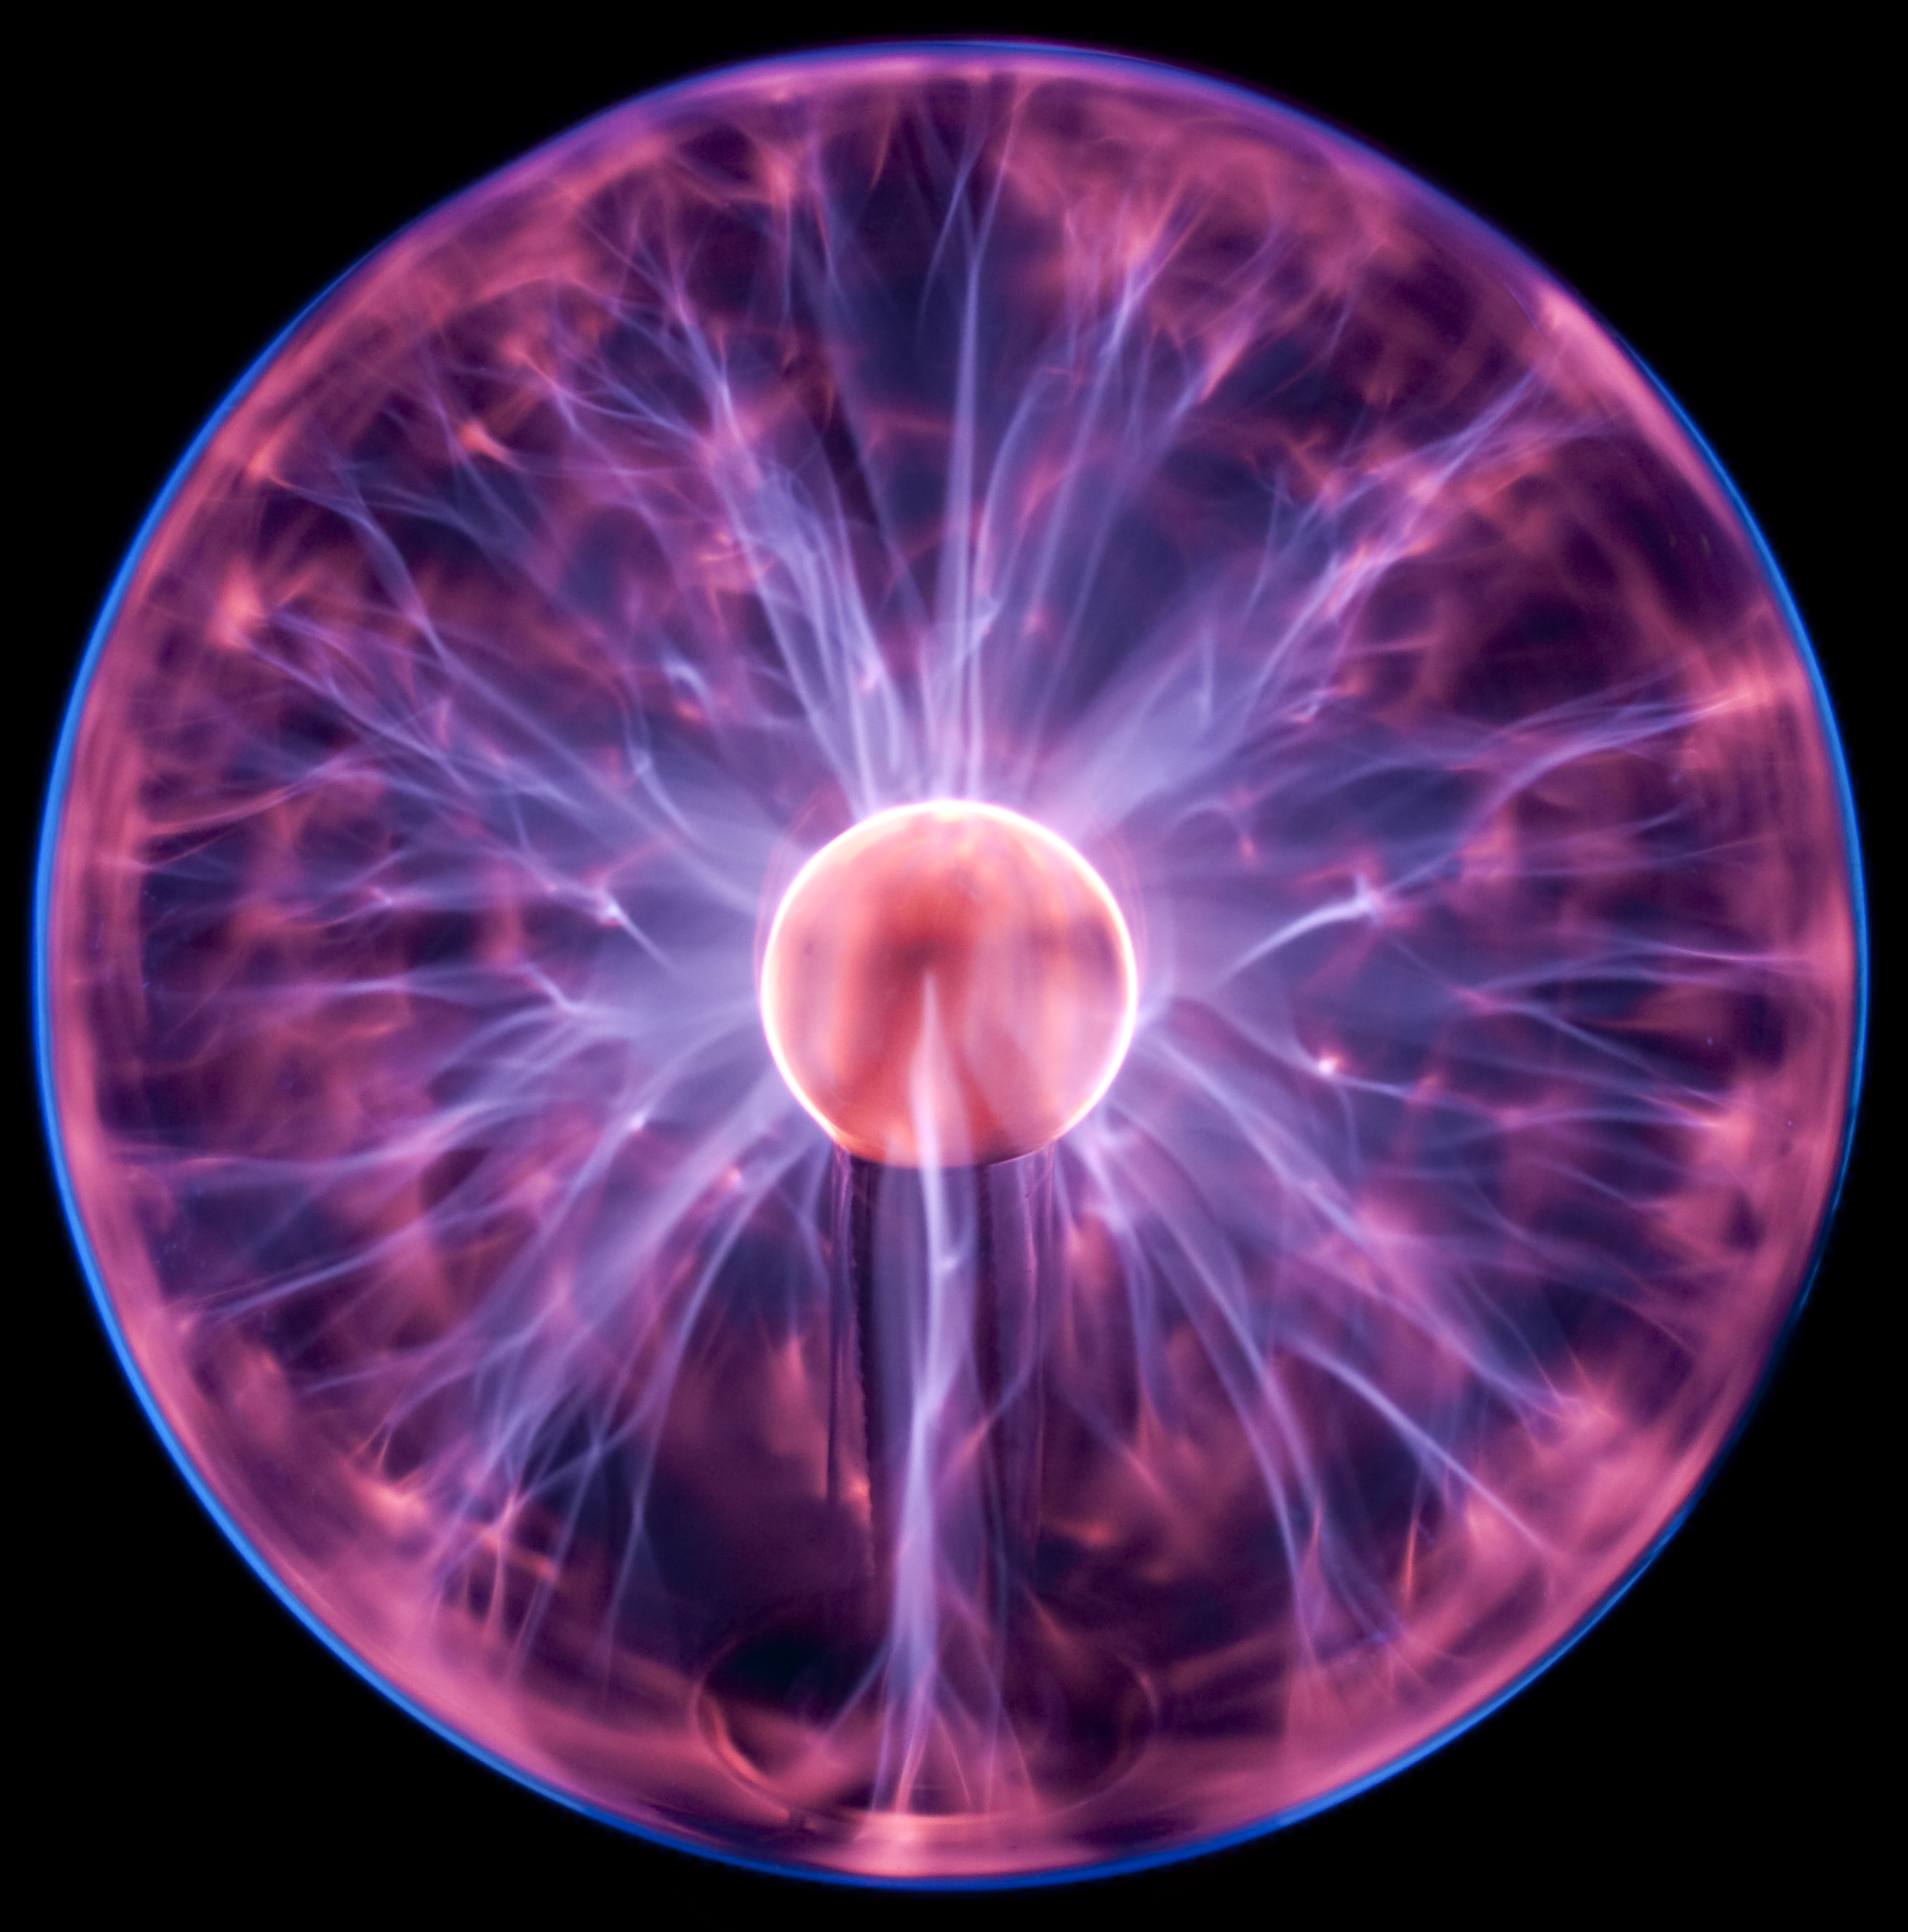
\includegraphics[width=.8\textwidth]{photos/plasmaball_by_ahisgett.jpg}\\
\textit{Photography by ahisgett on Flickr.}
\end{center}   
\end{minipage}
\begin{minipage}{.5\textwidth}
We use the symbol $I$ to show current and it is measured in amperes (A). One ampere is one coulomb of charge moving in one second ($\text{C} \cdot \text{s}^{-1}$).
\begin{equation*}
\boxed{I = \frac{Q}{\Delta t}}
\end{equation*}

When current flows in a circuit we show this on a diagram by adding arrows. The arrows show the direction of flow in a circuit. By convention we say that charge flows from the positive terminal on a battery to the negative terminal. 

If the voltage is high enough a current can be driven through almost anything. In the plasma ball example on the left, a voltage is created that is high enough to get charge to flow through the gas in the ball. The voltage is very high but the resulting current is very low. This makes it safe to touch.
\end{minipage}
\IFact{Benjamin Franklin made a guess about the
direction of charge flow when rubbing smooth wax with rough wool.
He thought that the charges flowed from the wax to the wool (i.e.
from positive to negative) which was opposite to the real
direction. Due to this, electrons are said to have a
\emph{negative} charge and so objects which Ben Franklin called
``negative'' (meaning a shortage of charge) really have an excess
of electrons. By the time the true direction of electron flow was
discovered, the convention of ``positive'' and ``negative'' had
already been so well accepted in the scientific world that no
effort was made to change it.}




\subsection*{Ammeter}

\begin{minipage}{.5\textwidth}
An ammeter is an instrument used to measure the rate of flow of electric
current in a circuit. Since one is interested in measuring the
current flowing \textit{through} a circuit component, the ammeter
must be connected in \textit{series} with the measured circuit
component.
\begin{center}
\begin{pspicture}(0,0)(3,3)
%\psgrid
\pnode(0,0){A} \pnode(0,2.5){B} \pnode(3,2.5){C} \pnode(3,0){D}
\battery[tension,dipoleconvention=generator](A)(B){$I$} \circledipole[labeloffset=0](B)(C){A}
\resistor[intensity,dipolestyle=rectangle](D)(C){} \wire[tension,arrowscale=2](D)(A)
\end{pspicture}
\label{fig:p:em:ec10:ammeter}
\end{center}
\end{minipage}
\begin{minipage}{.5\textwidth}
\begin{center}
\textbf{Ammeter}\\
%\includegraphics[width=.8\textwidth]{photos/ammeter_by_Hillwalker-ca_flickr.jpg}\\
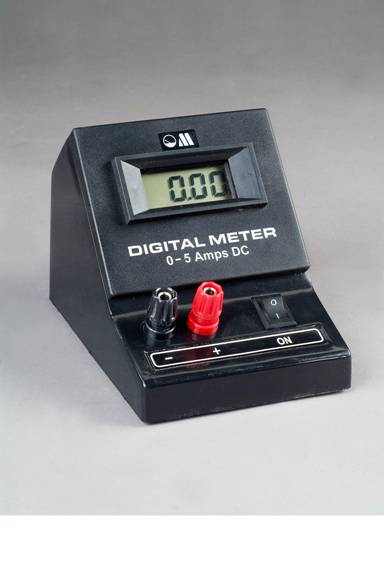
\includegraphics[width=.8\textwidth]{photos/type2ammeter.jpg}\\
%\textit{Photography by Hillwalker-ca on Flickr.}
\end{center}  
\end{minipage}

\begin{activity}{Constructing circuits}
%\begin{minipage}{.5\textwidth}
Construct circuits to measure the emf and the terminal potential difference for a battery.
% \end{minipage}
% \begin{minipage}{.5\textwidth}
%\subsubsection*{Components of electrical circuits}
Some common elements (components) which can be found in electrical circuits include light bulbs, batteries, connecting leads, switches, resistors, voltmeters and ammeters. You have learnt about many of these already. Below is a table with the items and their symbols:

\begin{table}[H]
\begin{center}
\begin{tabular}{|l|c|l|}\hline
\textbf{Component} & \textbf{Symbol} & \textbf{Usage} \\\hline\hline
\raisebox{0.35cm}{light bulb}&\begin{pspicture}(-0.5,-0.5)(0.5,0.5)
\scalebox{0.75}{\lamp(-1,0)(1,0){}}\end{pspicture} & 
\raisebox{0.35cm}{glows when charge moves through it} \\ \hline
\raisebox{0.35cm}{battery}&\begin{pspicture}(-0.5,-0.5)(0.5,0.5)
\scalebox{0.75}{\battery(-1,0)(1,0){}}\end{pspicture} & 
\raisebox{0.35cm}{provides energy for charge to move} \\ \hline
\raisebox{0.35cm}{switch}&\begin{pspicture}(-0.5,-0.5)(0.5,0.5)
\scalebox{0.75}{\switch(-1,0)(1,0){}}\end{pspicture} & 
\raisebox{0.35cm}{allows a circuit to be open or closed} \\ \hline
\raisebox{-0.35cm}{resistor}&\begin{pspicture}(-0.5,0)(0.5,0.5)
\scalebox{0.75}{\resistor(-1,0)(1,0){}}\end{pspicture} & 
\raisebox{-0.35cm}{resists the flow of charge} \\ 
&
OR& \\ 
&
\begin{pspicture}(-0.75,-0.25)(0.75,0.25)
\scalebox{0.75}{\resistor[dipolestyle=zigzag](-1,0)(1,0){}}\end{pspicture} & \\ \hline
\raisebox{0.35cm}{voltmeter}&\begin{pspicture}(-0.5,-0.5)(0.5,0.5)
\scalebox{0.75}{\circledipole[labeloffset=0](-1,0)(1,0){V}}\end{pspicture} & 
\raisebox{0.35cm}{measures potential difference} \\ \hline
\raisebox{0.35cm}{ammeter}&\begin{pspicture}(-0.5,-0.5)(0.5,0.5)
\scalebox{0.75}{\circledipole[labeloffset=0](-1,0)(1,0){A}}\end{pspicture} & 
\raisebox{0.35cm}{measures current in a circuit} \\ \hline
\raisebox{0.35cm}{connecting lead}&\begin{pspicture}(0,0)(1,1)
\psline(-0.25,0.5)(1.25,0.5)\end{pspicture} & 
\raisebox{0.35cm}{connects circuit elements together} \\ \hline
\hline
\end{tabular}
\end{center}
\end{table}
Experiment with different combinations of components in the circuits.

%\end{minipage}
\end{activity}
\Tip{A battery \textbf{does not} produce the same amount of
current no matter what is connected to it. While the voltage
produced by a battery is constant, the amount of current supplied
depends on what is in the circuit.}

The table below summarises the use of each measuring instrument
that we discussed and the way it should be connected to a circuit
component.

\begin{center}
\begin{tabular}{ | c | c | c | }
\hline 
\textbf{Instrument} & \textbf{Measured Quantity} & \textbf{Proper Connection} \\ \hline \hline 
Voltmeter & Voltage & In Parallel \\ \hline Ammeter &
Current & In Series \\ \hline
\hline
\end{tabular}
\end{center}


\begin{activity}{Using meters}If possible, 
connect meters in circuits to get used to the use of meters to
measure electrical quantities. If the meters have more than one
scale, always connect to the \textbf{largest scale} first so that the meter
will not be damaged by having to measure values that exceed its
limits.
\end{activity}



\begin{wex}{Calculating current I}
{An amount of charge equal to 45 C moves past a point in a circuit in 1 second, what is the current in the circuit?
}{%
\westep{Analyse the question}
We are given an amount of charge and a time and asked to calculate the current. We know that current is the rate at which charge moves past a fixed point in a circuit so we have all the information we need. We have quantities in the correct units already.
\westep{Apply the principles}
We know that:
\begin{eqnarray*}
I &=& \frac{Q}{\Delta t} \\
I &=& \frac{45~\text{C}}{1~\text{s}} \\
I &=& 45~\text{C} \cdot \text{s}^{-1} \\
I &=& 45~\text{A} \\
\end{eqnarray*}
\westep{Quote the final result}
The current is 45~A.
}
\end{wex}

\begin{wex}{Calculating current II}
{An amount of charge equal to 53 C moves past a fixed point in a circuit in 2 seconds, what is the current in the circuit?
}{%
\westep{Analyse the question}
We are given an amount of charge and a time and asked to calculate the current. We know that current is the rate at which charge moves past a fixed point in a circuit so we have all the information we need. We have quantities in the correct units already.
\westep{Apply the principles}
We know that:
\begin{eqnarray*}
I &=& \frac{Q}{\Delta t} \\
I &=& \frac{53~\text{C}}{2~\text{s}} \\
I &=& 26,5~\text{C} \cdot \text{s}^{-1} \\
I &=& 26,5~\text{A} \\
\end{eqnarray*}
\westep{Quote the final result}
The current is 26,5~A.
}
\end{wex}

\begin{wex}{Calculating current III}
{95 electrons move past a fixed point in a circuit in one tenth of a second, what is the current in the circuit?
}{%
\westep{Analyse the question}
We are given a number of charged particles that move past a fixed point and the time that it takes.
We know that current is the rate at which charge moves past a fixed point in a circuit so we have to determine the 
charge. In the last chapter we learnt that the charge carried by an electron is $1,6\times10^{-19}~\text{C}$.
\westep{Apply the principles: determine the charge}
We know that each electron carries a charge of $1,6\times10^{-19}~\text{C}$, therefore the total charge is:
\begin{eqnarray*}
Q & = & 95 \times 1,6\times10^{-19}~\text{C} \\
& = & 1,52\times10^{-17}~\text{C} 
\end{eqnarray*}
\westep{Apply the principles: determine the charge}
We know that:
\begin{eqnarray*}
I &=& \frac{Q}{\Delta t} \\
I &=& \frac{1,52\times10^{-17}~\text{C}}{\frac{1}{10}~\text{s}} \\
I &=& \frac{1,52\times10^{-17}~\text{C}}{1}\times{\frac{1}{{\frac{1}{10}~\text{s}}}} \\
I &=& \frac{1,52\times10^{-17}~\text{C}}{1}\times\frac{10}{1~\text{s}} \\
I &=& 1,52\times10^{-16}~\text{C} \cdot \text{s}^{-1} \\
I &=& 1,52\times10^{-16}~\text{A} \\
\end{eqnarray*}
\westep{Quote the final result}
The current is $1,52\times10^{-16}$~A.
}
\end{wex}


\section{Resistance}

Resistance is a measure of "how hard" it is to "push" electricity through a circuit element. Resistance can also apply to an entire circuit.

\subsection*{What causes resistance?}

\begin{minipage}{.5\textwidth}
On a microscopic level, electrons moving through
the conductor collide (or interact) with the particles of which the conductor
(metal) is made. When they collide, they transfer kinetic energy. 
The electrons therefore lose kinetic energy and slow down. This leads to
resistance. The transferred energy causes the resistor to heat up.
You can feel this directly if you touch a cellphone charger when you are charging a cell phone - the charger gets warm because its circuits have some resistors in them!
\end{minipage}
\begin{minipage}{.5\textwidth}
\begin{center}
 Examples of resistors\\
\includegraphics[width=.8\textwidth]{photos/resistors_oskay.jpg}\\
\textit{Photograph by oskay on Flickr}
\end{center}
\end{minipage}

\Definition{Resistance}{Resistance slows down the flow of charge in a circuit. The units of resistance are the ohm ($\Omega$) which is defined as a volt per ampere of current. \\
Symbol: $R$\hspace{2cm} Unit: Ohm ($\Omega$)\hspace{2cm}S.I. Units: $\text{m}^2\cdot\text{kg}\cdot\text{s}^{-3}\cdot\text{A}^{-2}$\\
}
\begin{equation*}
1 \ \text{Ohm} = 1 \frac{\text{Volt}}{ \text{Ampere}}
\end{equation*}

\IFact{Fluorescent lightbulbs do not use thin wires; they use the fact that certain gases glow when a current flows through them. They are much more efficient (much less resistance) than lightbulbs.} 

\begin{minipage}{.5\textwidth}
\begin{center}
Light bulb filament\\
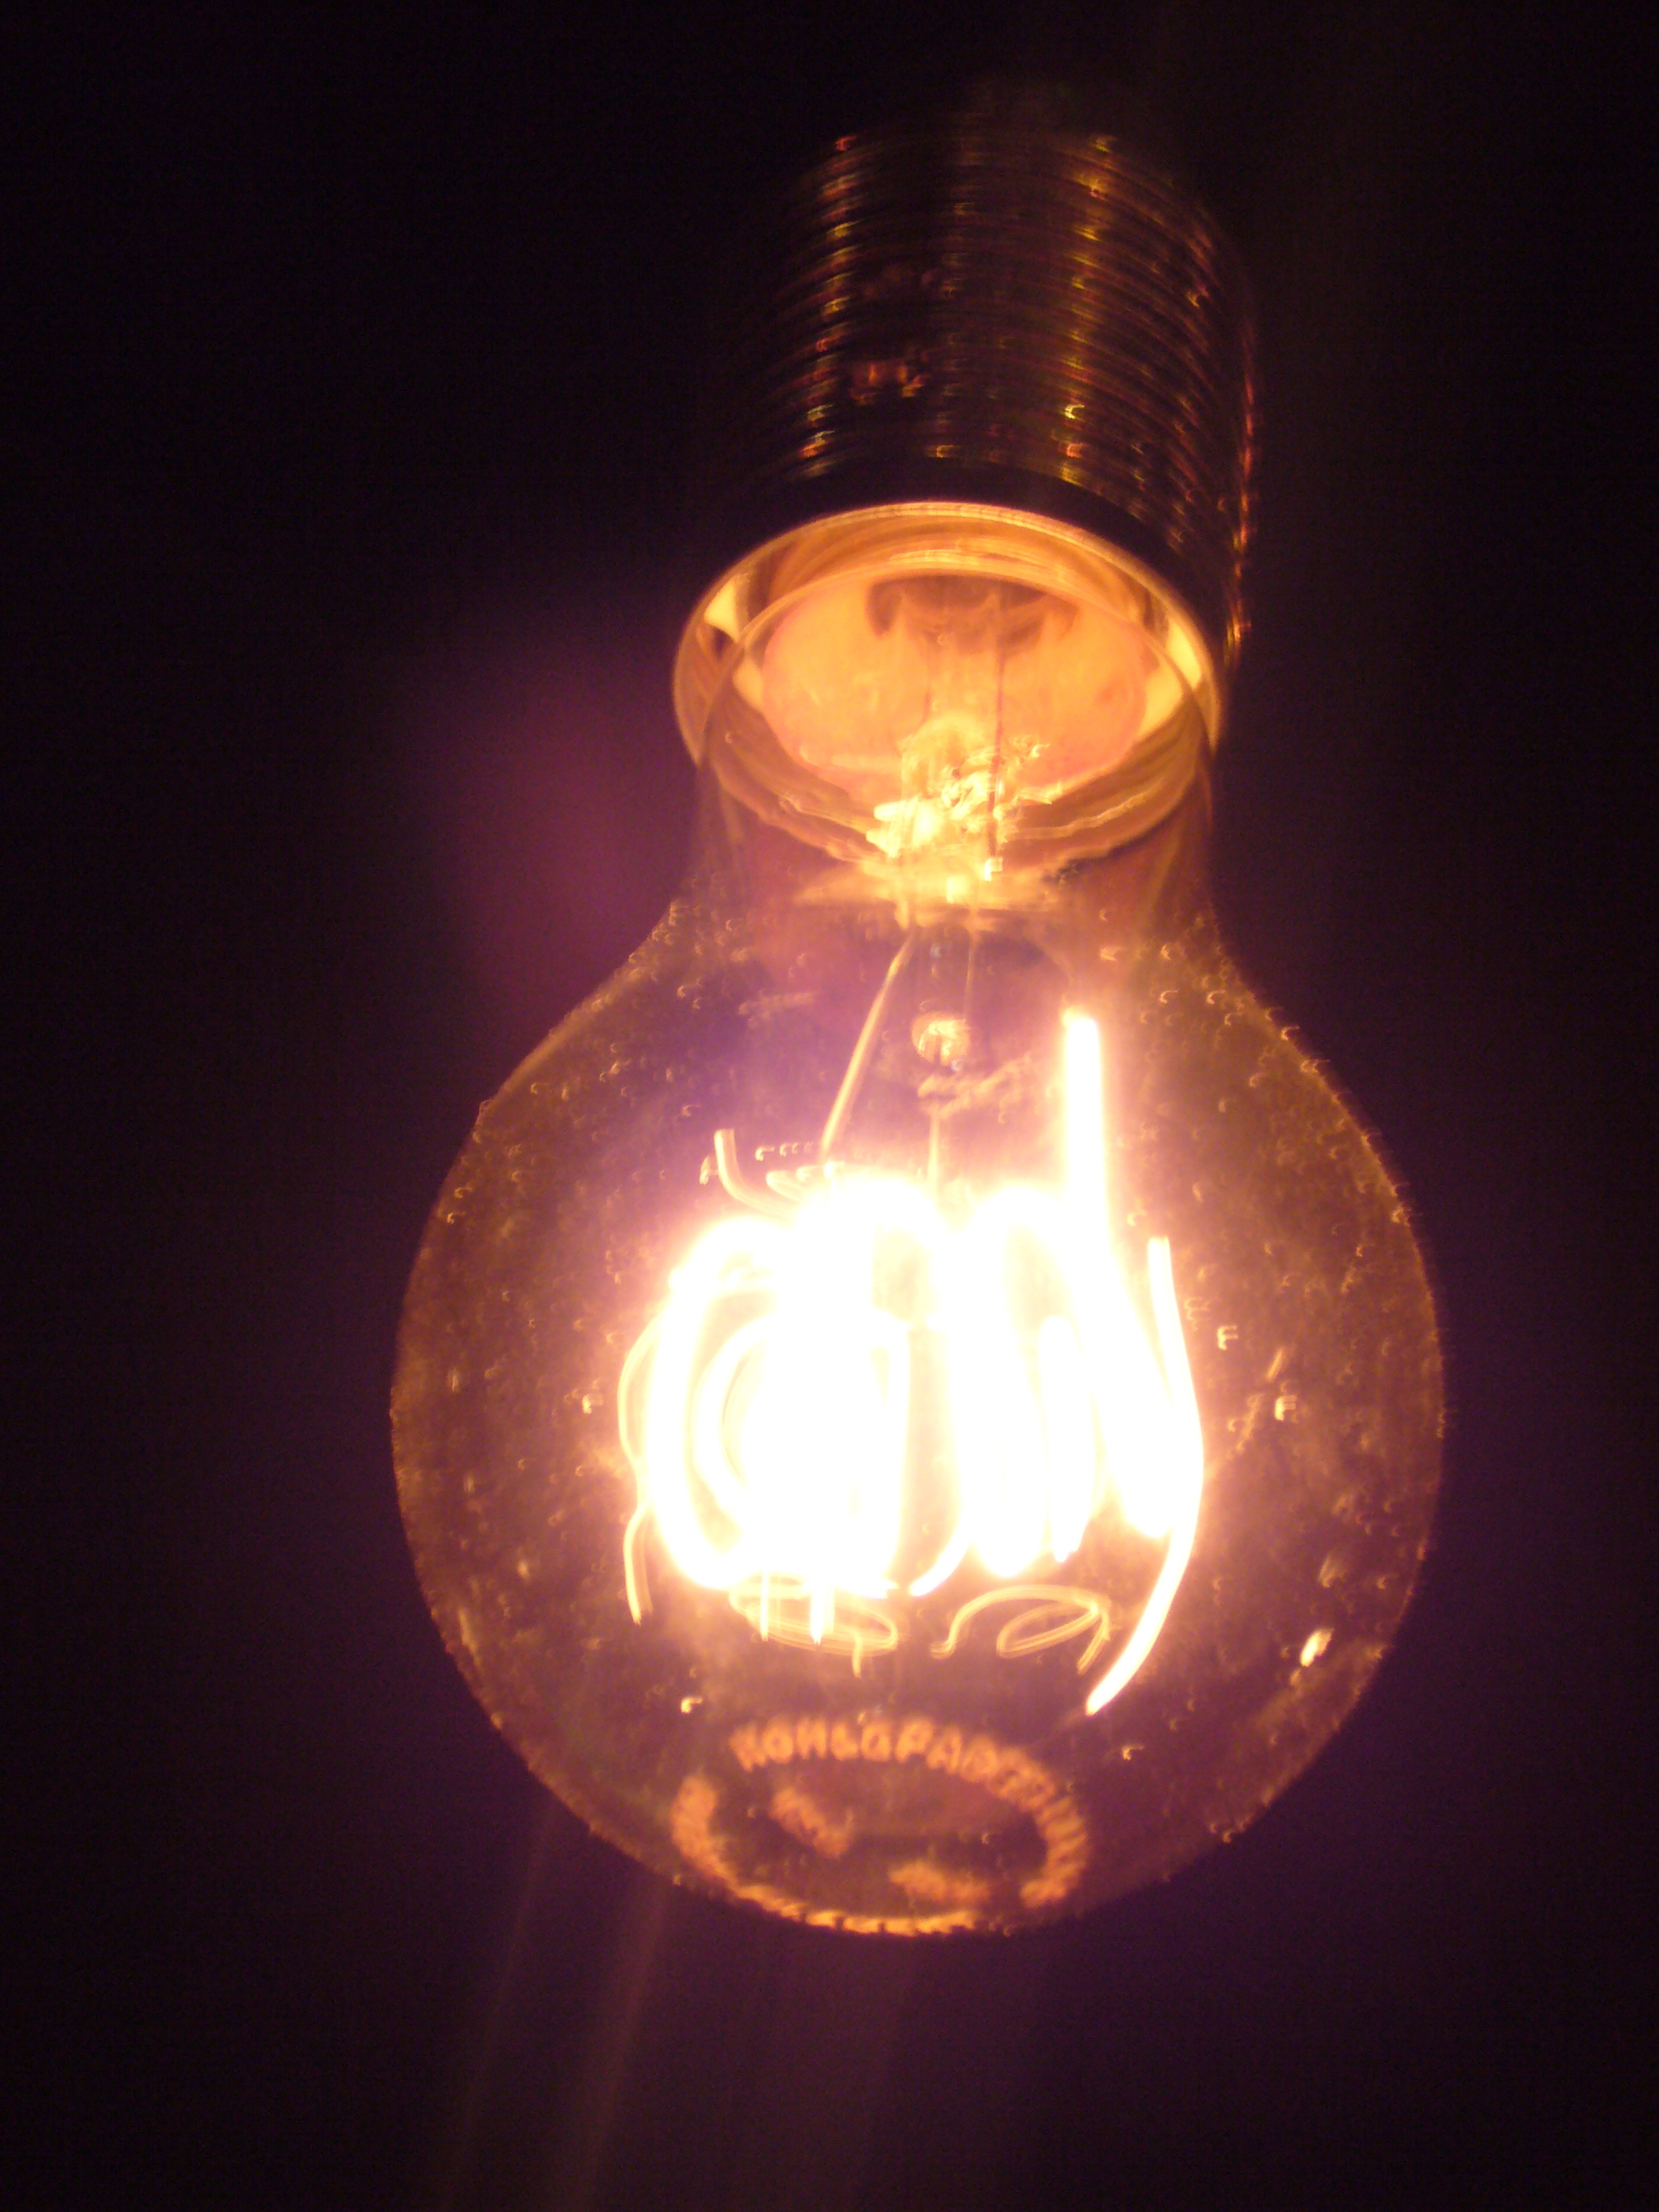
\includegraphics[width=.55\textwidth]{photos/lightbulb_by_clagnut.jpg}\\
\textit{Photography by clagnut on Flickr.}
\end{center}  
\end{minipage}
\begin{minipage}{.5\textwidth}

\textit{All} conductors have some resistance. For example, a piece of wire
has less resistance than a light bulb, but both have resistance. \\

A lightbulb is a very thin wire surrounded by a glass housing The high resistance of the small wire (filament) in a lightbulb causes the electrons to 
transfer a lot of their kinetic energy in the form of heat. The heat energy is enough
to cause the filament to glow white-hot which produces light.

\end{minipage}

The wires
connecting the lamp to the cell or battery hardly even get warm while
conducting the same amount of current. This is because of their
much lower resistance due to their larger cross-section (they are thicker).

An important effect of a resistor is that it \textit{converts} electrical
energy into other forms of \textbf{heat} energy. \textbf{Light} energy is a by-product of the heat that is produced.

\IFact{There is a special type of conductor,
called a \textbf{superconductor} that has no resistance, but the
materials that make up all known superconductors only start superconducting
at very low temperatures. The ``highest'' temperature superconductor is mercury barium calcium copper oxide (HgBa$_2$Ca$_2$Cu$_3$O$_x$) which is superconducting for temperatures of -140$^{o}$~C and colder.}

\subsubsection{Physical attributes affecting resistance}

The physical attributes of a resistor affect its total resistance.
\begin{itemize}
 \item \textbf{Length}: if a resistor is increased in length its resistance will increase. Typically if you increase the length of a resistor by a certain factor you will increase the resistance by the same factor.
\item \textbf{Width and height or cross-sectional area}: if a resistor provides a larger pathway by being made wider or broader then more current can flow through it. If the total surface area through which current flows (cross-sectional area) is increased by a factor the resistance typically decreases by the same factor. 
\end{itemize}
\textbf{Extension:}For a single resistor this can be summarised as
\begin{equation*}
 R\propto\frac{L}{A},
\end{equation*} where $L$ is the length and $A$ is the cross-sectional area.

\subsubsection*{Why do batteries go flat?}
A battery stores chemical potential energy. When it is connected in a circuit, a chemical reaction takes place inside the battery which converts chemical potential energy to electrical energy which powers the electrons to move through the circuit. All the circuit elements (such as the conducting leads, resistors and lightbulbs) have some resistance to the flow of charge and convert the electrical energy to heat and, in the case of the lightbulb, light.
Since energy is always conserved, the battery goes flat when all its chemical potential energy has been converted into other forms of energy.

\subsection*{Resistors in electric circuits}
It is important to understand what effect adding resistors to a circuit has on the \textit{total} resistance of a circuit and on the current that can flow in the circuit. 


\section{Potential difference and series resistors}

When resistors are in series, one after the other, there is a potential difference across each resistor. The total potential difference across a set of resistors in series is the sum of the potential differences across each of the resistors in the set. 
% This is the same as falling a large distance under gravity or falling that same distance (difference) in many smaller steps. The total distance (difference) is the same.

Look at the circuits below. If we measured the potential difference between the black dots in all of these circuits it would be the same as we saw earlier. So we now know the total potential difference is the same across one, two or three resistors. We also know that some work is required to make charge flow through each resistor.

\begin{center}
\begin{pspicture}(0,-0.5)(12,3.5)
%\psgrid
\pnode(0,0){A}
\pnode(0,3){B}
\pnode(3,3){C}
\pnode(3,0){D}
\psdot[dotscale=2](A)
\psdot[dotscale=2](B)

% draw battery and wires

\battery(A)(B){}
\psline(B)(C)
\psline(A)(D)

% draw resistors

\resistor[dipolestyle=rectangle](C)(D){}

% Second case
\rput(4,0){
% draw battery and wires
\pnode(0,0){A}
\pnode(0,3){B}
\pnode(3,3){C}
\pnode(3,0){D}

\battery(A)(B){}
\psline(B)(C)

\psdot[dotscale=2](A)
\psdot[dotscale=2](B)



% draw resistors

\resistor[dipolestyle=rectangle](C)(D){}
\resistor[dipolestyle=rectangle](A)(D){}
%\resistor[dipolestyle=rectangle](H)(J){}
}

% Third case
\rput(8,0){
% draw battery and wires
\pnode(0,0){A}
\pnode(0,3){B}
\pnode(3,3){C}
\pnode(3,0){D}
\pnode(3,2.5){E}
\pnode(3,.5){F}
\pnode(2,2.5){G}
\pnode(4,2.5){H}
\pnode(2,.5){I}
\pnode(4,.5){J}

\battery(A)(B){}

\psdot[dotscale=2](A)
\psdot[dotscale=2](B)


% draw resistors

\resistor[dipolestyle=rectangle](A)(D){}
\resistor[dipolestyle=rectangle](D)(C){}
\resistor[dipolestyle=rectangle](B)(C){}
}

\end{pspicture}
\end{center}

Let us look at this in a bit more detail. In the picture below you can see what the different measurements for 3 identical resistors in series could look like. The total voltage across all three resistors is the sum of the voltages across the individual resistors. Resistors in series are known as \texbf{voltage dividers} because the total voltage across all the resistors is divided amongst the individual resistors.

\begin{center}
\begin{pspicture}(0,-3.4525)(13.355,3.4325)
\psline[linewidth=0.04cm](1.88,1.3325)(1.88,0.3525)
\psline[linewidth=0.04cm](2.0,0.9725)(2.0,0.5925)
\psframe[linewidth=0.04,dimen=outer](1.14,-0.5075)(0.42,-0.8275)
\psframe[linewidth=0.04,dimen=outer](2.24,-0.5075)(1.52,-0.8275)
\psframe[linewidth=0.04,dimen=outer](3.32,-0.5075)(2.6,-0.8275)
\psline[linewidth=0.04cm](0.42,-0.6675)(0.02,-0.6675)
\psline[linewidth=0.04cm](0.02,-0.6675)(0.04,0.8525)
\psline[linewidth=0.04cm](0.04,0.8525)(1.82,0.8525)
\psline[linewidth=0.04cm](3.72,-0.6875)(3.32,-0.6875)
\psline[linewidth=0.04cm](3.7,-0.7075)(3.72,0.8125)
\psline[linewidth=0.04cm](3.72,0.8125)(2.08,0.8125)
\psline[linewidth=0.04cm](1.12,-0.6875)(1.52,-0.6875)
\psline[linewidth=0.04cm](2.22,-0.6875)(2.62,-0.6875)
\psline[linewidth=0.04cm](7.86,3.4125)(7.86,3.4125)
\psframe[linewidth=0.04,dimen=outer](7.68,0.0925)(6.96,-0.2275)
\psframe[linewidth=0.04,dimen=outer](9.4,0.0925)(8.68,-0.2275)
\psframe[linewidth=0.04,dimen=outer](11.1,0.0925)(10.38,-0.2275)
\psline[linewidth=0.04cm](7.64,-0.0675)(8.68,-0.0675)
\psline[linewidth=0.04cm](9.38,-0.0675)(10.42,-0.0675)
\psline[linewidth=0.04cm](6.96,-0.0675)(6.46,-0.0675)
\psline[linewidth=0.04cm](6.46,-0.0675)(6.46,0.9525)
\psline[linewidth=0.04cm](11.58,-0.0675)(11.08,-0.0675)
\psline[linewidth=0.04cm](11.58,-0.0675)(11.58,0.9525)
\psline[linewidth=0.04cm,linestyle=dashed,dash=0.16cm 0.16cm](6.46,0.9125)(6.46,1.6525)
\psline[linewidth=0.04cm,linestyle=dashed,dash=0.16cm 0.16cm](11.58,0.8925)(11.58,1.6325)
\psdots[dotsize=0.12](6.7,-0.0675)
\psdots[dotsize=0.12](7.92,-0.0675)
\psdots[dotsize=0.12](8.44,-0.0675)
\psdots[dotsize=0.12](9.64,-0.0675)
\psdots[dotsize=0.12](10.12,-0.0675)
\psdots[dotsize=0.12](11.38,-0.0475)
\pscircle[linewidth=0.04,dimen=outer](7.31,-1.0175){0.29}
\rput(7.31375,-1.0575){V}
\pscircle[linewidth=0.04,dimen=outer](9.05,-1.0175){0.29}
\rput(9.05375,-1.0575){V}
\pscircle[linewidth=0.04,dimen=outer](10.75,-1.0175){0.29}
\rput(10.75375,-1.0575){V}
\psbezier[linewidth=0.03](6.631698,-0.0875)(6.04,-0.6934091)(6.68,-1.1675)(7.02,-1.0875)
\psbezier[linewidth=0.03](7.928302,-0.0875)(8.52,-0.6934091)(7.88,-1.1675)(7.54,-1.0875)
\psbezier[linewidth=0.03](11.388302,-0.0875)(11.98,-0.6934091)(11.34,-1.1675)(11.0,-1.0875)
\psbezier[linewidth=0.03](10.131698,-0.0475)(9.54,-0.65340906)(10.18,-1.1275)(10.52,-1.0475)
\psbezier[linewidth=0.03](8.4,-0.0675)(7.92,-0.8309483)(8.66,-0.9275)(8.76,-0.94267243)
\psbezier[linewidth=0.03](9.66,-0.0875)(10.14,-0.8509483)(9.4,-0.9475)(9.3,-0.9626724)
\pscircle[linewidth=0.04,dimen=outer](9.03,-2.7975){0.29}
\rput(9.03375,-2.8375){V}
\psbezier[linewidth=0.03](6.68,-0.0475)(4.7,-1.5109637)(7.24,-2.7675)(8.74,-2.7964385)
\psbezier[linewidth=0.03](11.36,-0.0675)(13.34,-1.5309637)(10.8,-2.7875)(9.3,-2.8164384)
\rput(7.3184376,-1.5025){\scriptsize V = 5V}
\rput(9.038438,-1.5025){\scriptsize V = 5V}
\rput(10.758437,-1.5025){\scriptsize V = 5V}
\rput(9.128437,-3.3225){\scriptsize V = 15V}
\psline[linewidth=0.04cm,linestyle=dashed,dash=0.16cm 0.16cm,arrowsize=0.05291667cm 2.0,arrowlength=1.4,arrowinset=0.4]{->}(3.82,-0.7275)(6.3,-0.0075)
\rput(4.915781,-0.0225){\scriptsize zooming in}
\end{pspicture}
\end{center}

% \subsection*{Ohm's law}
% 
% The voltage is the change in potential energy or work done when charge moves between two points in the circuit. The greater the resistance to charge moving the more work that needs to be done. The work done or voltage thus depends on the resistance. The potential difference is proportional to the resistance.

% \Definition{Ohm's Law}{Voltage across a circuit component is proportional to the resistance of the component.}

% Use the fact that voltage is proportional to resistance to calculate what proportion of the total voltage of a circuit will be found across each circuit element. 

\subsubsection*{Resistors in series}
When we add resistors in series to a circuit, we \textit{increase} the resistance to the flow of current. There is only \textbf{one path} that the current can flow down and the current is the same at all places in the series circuit. Take a look at the diagram below. On the left there is a circuit with a single resistor and a battery. No matter where we measure the current, it is the same in a series circuit. On the right, we have added a second resistor in series to the circuit. The \textit{total} resistance of the circuit has \textit{increased} and you can see from the reading on the ammeter that the current in the circuit has decreased.

\begin{center}
\scalebox{1} % Change this value to rescale the drawing.
{
\begin{pspicture}(0,-2.43)(15.033594,2.43)
\psline[linewidth=0.04cm](8.128563,-0.127)(9.108562,-0.127)
\psline[linewidth=0.068cm](8.448563,-0.0070)(8.828563,-0.0070)
\psframe[linewidth=0.04,dimen=outer](11.34,1.99)(10.251562,1.53)
\rput(7.99,-0.385){\small V = 2 V}
\rput(10.802188,2.235){\small R = 2 $\Omega$}
\rput(14.283594,0.475){\small I = 0.67 A}
\rput(10.840313,-1.805){Adding a resistor to the circuit }
\rput(10.866406,-2.225){increases the total resistance}
\psframe[linewidth=0.04,dimen=outer](11.28,-0.97)(10.191563,-1.43)
\pscircle[linewidth=0.04,dimen=outer](13.05,0.44){0.39}
\pscircle[linewidth=0.04,dimen=outer](8.69,1.02){0.39}
\rput(8.72,1.06){\large A}
\rput(13.06,0.44){\large A}
\psline[linewidth=0.04cm](8.64,0.03)(8.64,0.65)
\psline[linewidth=0.04cm](8.68,1.37)(8.66,1.75)
\psline[linewidth=0.04cm](8.66,1.75)(10.28,1.75)
\psline[linewidth=0.04cm](11.34,1.77)(13.08,1.77)
\psline[linewidth=0.04cm](13.1,1.77)(13.1,0.79)
\psline[linewidth=0.04cm](13.08,0.07)(13.08,-1.23)
\psline[linewidth=0.04cm](13.1,-1.21)(11.26,-1.21)
\psline[linewidth=0.04cm](8.64,-0.11)(8.64,-1.19)
\psline[linewidth=0.04cm](8.62,-1.19)(10.22,-1.19)
\rput(10.762188,-0.745){\small R = 1 $\Omega$}
\rput(9.843594,0.995){\small I = 0.67 A}
\psline[linewidth=0.04cm](0.6885625,-0.127)(1.6685625,-0.127)
\psline[linewidth=0.068cm](1.0085624,-0.0070)(1.3885624,-0.0070)
\psframe[linewidth=0.04,dimen=outer](3.9,1.99)(2.8115625,1.53)
\rput(0.55,-0.385){\small V = 2 V}
\rput(3.3621874,2.235){\small R = 2 $\Omega$}
\rput(6.563594,0.455){\small I = 1 A}
\rput(3.4703126,-1.825){The current in a series circuit }
\rput(3.3664062,-2.205){is the same everywhere}
\pscircle[linewidth=0.04,dimen=outer](5.61,0.44){0.39}
\pscircle[linewidth=0.04,dimen=outer](1.25,1.02){0.39}
\rput(1.28,1.06){\large A}
\rput(5.62,0.44){\large A}
\psline[linewidth=0.04cm](1.2,0.03)(1.2,0.65)
\psline[linewidth=0.04cm](1.24,1.37)(1.22,1.75)
\psline[linewidth=0.04cm](1.22,1.75)(2.84,1.75)
\psline[linewidth=0.04cm](3.9,1.77)(5.64,1.77)
\psline[linewidth=0.04cm](5.66,1.77)(5.66,0.79)
\psline[linewidth=0.04cm](5.64,0.07)(5.64,-1.23)
\psline[linewidth=0.04cm](1.2,-0.11)(1.2,-1.19)
\psline[linewidth=0.04cm](1.18,-1.19)(5.66,-1.19)
\rput(2.183594,0.995){\small I = 1 A}
\rput(14.106406,-0.11){\footnotesize (the current is }
\rput(13.746407,-0.41){\footnotesize smaller)}
\rput(9.626407,0.35){\footnotesize smaller)}
\rput(9.986406,0.65){\footnotesize (the current is }
\end{pspicture} 
}
\end{center}

\begin{g_experiment}{Voltage dividers}
 
\textbf{Aim:} Test what happens to the current and the voltage in series circuits when additional resistors are added.\\
\textbf{Apparatus:}\begin{itemize}
                    \item A battery
		    \item A voltmeter
		    \item An ammeter
		    \item Wires
		    \item Resistors
                   \end{itemize}
\textbf{Method:}\begin{itemize}
                 \item Construct each circuit shown below
		  \item Measure the voltage across each resistor in the circuit.
		  \item Measure the current before and after each resistor in the circuit.
                \end{itemize}
\begin{center}
\begin{pspicture}(0,-0.5)(12,3.5)
%\psgrid
\pnode(0,0){A}
\pnode(0,3){B}
\pnode(3,3){C}
\pnode(3,0){D}
\psdot[dotscale=2](A)
\psdot[dotscale=2](B)

% draw battery and wires

\battery(A)(B){}
\psline(B)(C)
\psline(A)(D)

% draw resistors

\resistor[dipolestyle=rectangle](C)(D){$\rm{R}_{1}$}

% Second case
\rput(4.5,0){
% draw battery and wires
\pnode(0,0){A}
\pnode(0,3){B}
\pnode(3,3){C}
\pnode(3,0){D}

\battery(A)(B){}
\psline(B)(C)

\psdot[dotscale=2](A)
\psdot[dotscale=2](B)



% draw resistors

\resistor[dipolestyle=rectangle](C)(D){$\rm{R}_{1}$}
\resistor[dipolestyle=rectangle](A)(D){$\rm{R}_{2}$}
%\resistor[dipolestyle=rectangle](H)(J){}
}

% Third case
\rput(9,0){
% draw battery and wires
\pnode(0,0){A}
\pnode(0,3){B}
\pnode(3,3){C}
\pnode(3,0){D}
\pnode(3,2.5){E}
\pnode(3,.5){F}
\pnode(2,2.5){G}
\pnode(4,2.5){H}
\pnode(2,.5){I}
\pnode(4,.5){J}

\battery(A)(B){}

\psdot[dotscale=2](A)
\psdot[dotscale=2](B)


% draw resistors

\resistor[dipolestyle=rectangle](A)(D){$\rm{R}_{2}$}
\resistor[dipolestyle=rectangle](D)(C){$\rm{R}_{1}$}
\resistor[dipolestyle=rectangle](B)(C){$\rm{R}_{3}$}
}
\end{pspicture}
\end{center}
\textbf{Results and conclusions:} \begin{itemize}
                   \item Compare the sum of the voltages across all the resistors in each of the circuits.
		    \item Compare the various current measurements within the same circuit.
                  \end{itemize}

\end{g_experiment}

The total resistance is equal to $\rm{R}_{1}$ in the first circuit, to $\rm{R}_{1}$ + $\rm{R}_{2}$ in the second circuit and $\rm{R}_{1}$ + $\rm{R}_{2}$ + $\rm{R}_{3}$ in the third circuit.
In general, for resistors in series, the total resistance is given by:
\begin{equation*}
 R_S = R_1 + R_2 + \ldots
\end{equation*}

We know that the potential energy lost across a resistor is proportional to the resistance of the component because the higher the resistance the more work must be done to drive charge through the resistor.

\begin{wex}{Series resistors I}{%
A circuit contains two resistors in series. The resistors have resistance values of $5~\Omega$ and $17~\Omega$. \\
\begin{center}
\begin{pspicture}(-0.2,-0.2)(3.5,3.5)
\pnode(0,0){A}
\pnode(0,3){B}
\pnode(3,3){C}
\pnode(3,0){D}
\battery(A)(B){}
\psline(B)(C)
\psdot[dotscale=2](A)
\psdot[dotscale=2](B)
% draw resistors
\resistor[dipolestyle=rectangle](C)(D){$5~\Omega$}
\resistor[dipolestyle=rectangle](A)(D){$17~\Omega$}
%\resistor[dipolestyle=rectangle](H)(J){}
\end{pspicture}\end{center}\\
What is the total resistance in the circuit?}{%
\westep{Analyse the question}
We are told that the circuit is a series circuit and that we need to calculate the total resistance. The values of the two resistors have been given in the correct units, $\Omega$.
\westep{Apply the relevant principles}
The total resistance for resistors in series is the sum of the individual resistances. We can use
\begin{equation*}
 R_S = R_1 + R_2 + \ldots
\end{equation*}.
We have only two resistors and we now the resistances. In this case we have that:
\begin{align*}
 R_S &= R_1 + R_2 + \ldots\\
R_S &= R_1 + R_2\\
&=5~\Omega + 17~\Omega\\
&=22~\Omega
\end{align*}
\westep{Quote the final result}
The total resistance of the resistors in series is $22~\Omega$.}\end{wex}

\begin{wex}{Series resistors II}{
A circuit contains three resistors in series. The resistors have resistance values of $0,5~\Omega$, $7,5~\Omega$ and $11~\Omega$.
\begin{center}
\begin{pspicture}(-1,-1)(5.5,5.5)
%\psgrid
\pnode(0,0){A}
\pnode(0,3){B}
\pnode(3,3){C}
\pnode(3,0){D}
\battery(A)(B){}
% draw resistors
\resistor[dipolestyle=rectangle,labeloffset=1](C)(D){$0,5~\Omega$}
\resistor[dipolestyle=rectangle](A)(D){$7,5~\Omega$}
\resistor[dipolestyle=rectangle](B)(C){$11~\Omega$}
\end{pspicture}\end{center}\\
What is the total resistance in the circuit?}{%
\westep{Analyse the question}
We are told that the circuit is a series circuit and that we need to calculate the total resistance. The values of the three resistors have been given in the correct units, $\Omega$.
\westep{Apply the relevant principles}
The total resistance for resistors in series is the sum of the individual resistances. We can use
\begin{equation*}
 R_S = R_1 + R_2 + \ldots
\end{equation*}.
We have three resistors and we now the resistances. In this case we have that:
\begin{align*}
 R_S &= R_1 + R_2 + \ldots\\
R_S &= R_1 + R_2 + R_3\\
&=0,5~\Omega + 7,5~\Omega + 11~\Omega\\
&=19~\Omega
\end{align*}
\westep{Quote the final result}
The total resistance of the resistors in series is $19~\Omega$.}\end{wex}

\begin{wex}{Series resistors III}{%
A circuit contains two resistors in series. The resistors have resistance values of $750~k\Omega$ and $1,7~M\Omega$. \\
\begin{center}
\begin{pspicture}(-0.2,-0.2)(3.5,3.5)
\pnode(0,0){A}
\pnode(0,3){B}
\pnode(3,3){C}
\pnode(3,0){D}
\battery(A)(B){}
\psline(B)(C)
% \psdot[dotscale=2](A)
% \psdot[dotscale=2](B)
% draw resistors
\resistor[dipolestyle=rectangle,labeloffset=1](C)(D){$750~k\Omega$}
\resistor[dipolestyle=rectangle](A)(D){$1,7~M\Omega$}
%\resistor[dipolestyle=rectangle](H)(J){}
\end{pspicture}\end{center}\\
What is the total resistance in the circuit?}{%
\westep{Analyse the question}
We are told that the circuit is a series circuit and that we need to calculate the total resistance. The values of the two resistors have been given in the correct units, $\Omega$.
\westep{Apply the relevant principles}
The total resistance for resistors in series is the sum of the individual resistances. We can use
\begin{equation*}
 R_S = R_1 + R_2 + \ldots
\end{equation*}.
We have only two resistors and we now the resistances. In this case we have that:
\begin{align*}
 R_S &= R_1 + R_2 + \ldots\\
R_S &= R_1 + R_2\\
&=750~k\Omega + 1,7~M\Omega\\
&=750\times10^{3}~\Omega + 1,7\times10^{6}~\Omega\\
&=0,75\times10^{6}~\Omega + 1,7\times10^{6}~\Omega\\
&=2,45\times10^{6}~\Omega=2,45~M\Omega
\end{align*}
\westep{Quote the final result}
The total resistance of the resistors in series is $2,45~M\Omega$.}\end{wex}


\section{Potential difference and parallel resistors}

When resistors are connected in parallel the start and end points for all the resistors are the same. These points have the same potential energy and so the potential difference between them is the same no matter what is put in between them. You can have one, two or many resistors between the two points, the potential difference will not change. You can ignore whatever components are between two points in a circuit when calculating the difference between the two points.

%Test this by measuring the potential difference between points A and B in the following circuits.

Look at the following circuit diagrams. The battery is the same in all cases, all that changes is more resistors are added between the points marked by the black dots. If we were to measure the potential difference between the two dots in these circuits we would get the same answer for all three cases.

%\begin{figure}[htbp]
%\begin{center}
%\begin{pspicture}(0,0)(3,3)
%\psgrid
%\pnode(0,0){A}
%\pnode(0,2.5){B}
%\pnode(3,2.5){C}
%\pnode(3,0){D}
%\pnode(5,2.5){E}
%\pnode(5,0){F}
%\battery(A)(B){}
%\circledipole[labeloffset=0](E)(F){V}
%\resistor[dipolestyle=rectangle](C)(D){}
%\psline(D)(A)
%\end{pspicture}
%\caption{An ammeter should be connected in series in a circuit.}
%\label{fig:p:em:ec10:ammeter}
%\end{center}
%\end{figure}

\begin{center}
\begin{pspicture}(0,-0.5)(12,3.5)
%\psgrid
\pnode(0,0){A}
\pnode(0,3){B}
\pnode(3,3){C}
\pnode(3,0){D}
\pnode(3,2.5){E}
\pnode(3,.5){F}
\pnode(2,2.5){G}
\pnode(4,2.5){H}
\pnode(2,.5){I}
\pnode(4,.5){J}
\psdot[dotscale=2](C)
\psdot[dotscale=2](D)

% draw battery and wires

\battery(A)(B){}
\psline(B)(C)
\psline(C)(E)
\psline(A)(D)
\psline(D)(F)

% draw resistors

\resistor[dipolestyle=rectangle](E)(F){}
%\resistor[dipolestyle=rectangle](G)(I){}
%\resistor[dipolestyle=rectangle](H)(J){}

% Second case
\rput(4,0){
% draw battery and wires
\pnode(0,0){A}
\pnode(0,3){B}
\pnode(3,3){C}
\pnode(3,0){D}
\pnode(3,2.5){E}
\pnode(3,.5){F}
\pnode(2,2.5){G}
\pnode(4,2.5){H}
\pnode(2,.5){I}
\pnode(4,.5){J}



\battery(A)(B){}
\psline(B)(C)
\psline(C)(E)
\psline(A)(D)
\psline(D)(F)

\psline(E)(G)
\psline(F)(I)

\psdot[dotscale=2](C)
\psdot[dotscale=2](D)



% draw resistors

\resistor[dipolestyle=rectangle](E)(F){}
\resistor[dipolestyle=rectangle](G)(I){}
%\resistor[dipolestyle=rectangle](H)(J){}
}



% Third case
\rput(8,0){
% draw battery and wires
\pnode(0,0){A}
\pnode(0,3){B}
\pnode(3,3){C}
\pnode(3,0){D}
\pnode(3,2.5){E}
\pnode(3,.5){F}
\pnode(2,2.5){G}
\pnode(4,2.5){H}
\pnode(2,.5){I}
\pnode(4,.5){J}

\battery(A)(B){}
\psline(B)(C)
\psline(C)(E)
\psline(A)(D)
\psline(D)(F)

\psline(E)(G)
\psline(E)(H)
\psline(F)(I)
\psline(F)(J)

\psdot[dotscale=2](C)
\psdot[dotscale=2](D)


% draw resistors

\resistor[dipolestyle=rectangle](E)(F){}
\resistor[dipolestyle=rectangle](G)(I){}
\resistor[dipolestyle=rectangle](H)(J){}
}

\end{pspicture}
\end{center}

Lets look at two resistors in parallel more closely. When you construct a circuit you use wires and you might think that measuring the voltage in different places on the wires will make a difference. This is not true. The potential difference or voltage measurement will only be different if you measure a different set of components. All points on the wires that have no circuit components between them will give you the same measurements.

All three of the measurements shown in the picture below (i.e. A--B, C--D and E--F) will give you the same voltage. The different measurement points on the left have no components between them so there is no change in potential energy. 
Exactly the same applies to the different points on the right. When you measure the potential difference between the points on the left and right you will get the same answer.

\begin{center}
\begin{pspicture}(0,-2.9910936)(10.618125,2.9710937)
\psline[linewidth=0.04cm](1.078125,2.3310938)(1.078125,1.3510938)
\psline[linewidth=0.04cm](1.198125,1.9710938)(1.198125,1.5910938)
\psframe[linewidth=0.04,dimen=outer](1.458125,0.5910938)(0.738125,0.27109376)
\psframe[linewidth=0.04,dimen=outer](1.458125,-0.10890625)(0.738125,-0.42890626)
\psline[linewidth=0.04cm](1.258125,1.7710937)(2.118125,1.7710937)
\psline[linewidth=0.04cm](2.118125,1.7710937)(2.118125,0.05109375)
\psline[linewidth=0.04cm](1.638125,0.43109375)(1.438125,0.43109375)
\psline[linewidth=0.04cm](1.658125,-0.24890625)(1.458125,-0.24890625)
\psline[linewidth=0.04cm](0.738125,0.43109375)(0.518125,0.43109375)
\psline[linewidth=0.04cm](0.518125,0.43109375)(0.518125,-0.28890625)
\psline[linewidth=0.04cm](0.518125,-0.28890625)(0.758125,-0.28890625)
\psline[linewidth=0.04cm](0.498125,0.05109375)(0.138125,0.05109375)
\psline[linewidth=0.04cm](0.138125,0.05109375)(0.158125,1.7510937)
\psline[linewidth=0.04cm](0.158125,1.7510937)(1.058125,1.7510937)
\psline[linewidth=0.04cm](1.638125,0.41109374)(1.638125,-0.24890625)
\psline[linewidth=0.04cm](1.638125,0.03109375)(2.138125,0.05109375)
\usefont{T1}{ptm}{m}{n}
\rput(0.5990625,0.68109375){A}
\usefont{T1}{ptm}{m}{n}
\rput(1.670625,0.6610938){B}
\usefont{T1}{ptm}{m}{n}
\rput(0.49921876,-0.5389063){C}
\usefont{T1}{ptm}{m}{n}
\rput(1.6173438,-0.49890625){D}
\usefont{T1}{ptm}{m}{n}
\rput(0.04921875,-0.19890624){E}
\usefont{T1}{ptm}{m}{n}
\rput(2.0864062,-0.19890624){F}
\psline[linewidth=0.04cm,linestyle=dashed,dash=0.16cm 0.16cm,arrowsize=0.05291667cm 2.0,arrowlength=1.4,arrowinset=0.4]{->}(2.738125,-0.12890625)(5.418125,0.57109374)
\usefont{T1}{ptm}{m}{n}
\rput{13.4721575}(0.1506071,-0.9007815){\rput(3.8729484,0.6556103){zooming in:}}
\psline[linewidth=0.04cm](6.598125,0.57109374)(7.418125,1.2710937)
\psline[linewidth=0.04cm](6.598125,0.5910938)(7.418125,-0.10890625)
\psframe[linewidth=0.04,dimen=outer](8.138125,1.4310937)(7.418125,1.1110938)
\psframe[linewidth=0.04,dimen=outer](8.118125,0.07109375)(7.398125,-0.24890625)
\psline[linewidth=0.04cm](8.118125,-0.08890625)(8.938125,0.61109376)
\psline[linewidth=0.04cm](8.118125,1.2910937)(8.938125,0.5910938)
\psline[linewidth=0.04cm](6.598125,0.5910938)(6.238125,0.5910938)
\psline[linewidth=0.04cm](8.938125,0.5910938)(9.278125,0.5910938)
\usefont{T1}{ptm}{m}{n}
\rput(6.509219,0.32109374){E}
\usefont{T1}{ptm}{m}{n}
\rput(8.966406,0.32109374){F}
\usefont{T1}{ptm}{m}{n}
\rput(7.2590623,0.7810938){A}
\usefont{T1}{ptm}{m}{n}
\rput(8.250625,0.7810938){B}
\usefont{T1}{ptm}{m}{n}
\rput(7.1992188,0.28109375){C}
\usefont{T1}{ptm}{m}{n}
\rput(8.257343,0.28109375){D}
\psdots[dotsize=0.12](7.138125,1.0110937)
\psdots[dotsize=0.12](8.378125,1.0510937)
\psdots[dotsize=0.12](7.118125,0.13109376)
\psdots[dotsize=0.12](8.358125,0.11109375)
\psdots[dotsize=0.12](6.598125,0.5910938)
\psdots[dotsize=0.12](8.918125,0.5910938)
\pscircle[linewidth=0.04,dimen=outer](7.768125,1.9410938){0.29}
\usefont{T1}{ptm}{m}{n}
\rput(7.7721877,1.9010937){V}
\pscircle[linewidth=0.04,dimen=outer](7.748125,-0.69890624){0.29}
\usefont{T1}{ptm}{m}{n}
\rput(7.7521877,-0.73890626){V}
\pscircle[linewidth=0.04,dimen=outer](7.748125,-1.8789062){0.29}
\usefont{T1}{ptm}{m}{n}
\rput(7.7521877,-1.9189062){V}
\psbezier[linewidth=0.04](7.138125,1.0310937)(6.978125,1.2110938)(6.558125,2.1110938)(7.478125,1.9484271)
\psbezier[linewidth=0.04](8.378125,1.0710938)(8.538125,1.2510937)(8.958125,2.1510937)(8.038125,1.988427)
\psbezier[linewidth=0.04](7.078125,0.15109375)(6.258125,-0.28132004)(6.938125,-0.86890626)(7.458125,-0.7289063)
\psbezier[linewidth=0.04](8.358125,0.15109375)(9.178125,-0.28132004)(8.498125,-0.86890626)(7.978125,-0.7289063)
\psbezier[linewidth=0.04](6.598125,0.5910938)(4.898125,-0.98890626)(7.038125,-2.0489063)(7.498125,-1.8289063)
\psbezier[linewidth=0.04](8.898125,0.5910938)(10.598125,-0.98890626)(8.458125,-2.0489063)(7.998125,-1.8289063)
\usefont{T1}{ptm}{m}{n}
\rput(7.7801566,2.3560936){\scriptsize V = 5 V}
\usefont{T1}{ptm}{m}{n}
\rput(8.560157,-0.98390627){\scriptsize V = 5 V}
\usefont{T1}{ptm}{m}{n}
\rput(7.8001556,-2.3839064){\scriptsize V = 5 V}
\psline[linewidth=0.04cm](6.258125,0.5910938)(6.258125,2.0710938)
\psline[linewidth=0.04cm](9.278125,0.57109374)(9.278125,2.0510938)
\psline[linewidth=0.04cm,linestyle=dashed,dash=0.16cm 0.16cm](6.258125,2.0110939)(6.258125,2.9310937)
\psline[linewidth=0.04cm,linestyle=dashed,dash=0.16cm 0.16cm](9.278125,2.0310938)(9.278125,2.9510937)
\psdots[dotsize=0.12](0.518125,0.43109375)
\psdots[dotsize=0.12](0.518125,-0.26890624)
\psdots[dotsize=0.12](1.618125,-0.24890625)
\psdots[dotsize=0.12](1.638125,0.45109376)
\psdots[dotsize=0.12](2.078125,0.05109375)
\psdots[dotsize=0.12](0.138125,0.07109375)
\end{pspicture} 
\end{center}


\begin{wex}{Voltages I}{
Consider this circuit diagram:\\
\begin{center}
\begin{pspicture}(-3,-0.5)(3,3.5)
%\psgrid
\pnode(0,0){A}
\pnode(0,3){B}
\pnode(3,3){C}
\pnode(3,0){D}
% draw battery and wires
\battery(A)(B){2\text{V}}
\psline(B)(C)
\psline(A)(D)
% draw resistors
\resistor[dipolestyle=rectangle](C)(D){$\rm{V}_{1}$}
\end{pspicture}\end{center}\\
What is the voltage across the resistor in the circuit shown?
}{%
\westep{Check what you have and the units}
We have a circuit with a battery and one resistor. We know the voltage across the battery. We want to find that voltage across the resistor.
\begin{equation*}
V_{battery} = 2~\text{V}
\end{equation*}

\westep{Applicable principles}
We know that the voltage across the battery must be equal to the total voltage across all other circuit components. 
\begin{equation*}
V_{battery} = V_{total}
\end{equation*}
There is only one other circuit component, the resistor. 
\begin{equation*}
V_{total} = V_{1}
\end{equation*}
This means that the voltage across the battery is the same as the voltage across the resistor.
\begin{equation*}
V_{battery} = V_{total} = V_{1}
\end{equation*}
\begin{equation*}
V_{battery} = V_{total} = V_{1}
\end{equation*}
\begin{equation*}
V_{1} = 2\rm{V}
\end{equation*}}\end{wex}
\clearpage

\begin{wex}{Voltages II}{
Consider this circuit:\\
\begin{pspicture}(-3,-0.5)(3,3.5)
%\psgrid
\pnode(0,0){A}
\pnode(0,3){B}
\pnode(3,3){C}
\pnode(3,0){D}
% \psdot[dotscale=2](A)
% \psdot[dotscale=2](B)
% draw battery and wires
\battery(A)(B){2V}
\psline(B)(C)
% draw resistors
\resistor[dipolestyle=rectangle](A)(D){$V_{\rm{B}}=1$V}
\resistor[dipolestyle=rectangle](C)(D){$V_{\rm{A}}$}
\end{pspicture}\\
What is the voltage across the unknown resistor in the circuit shown?
}%
{%
\westep{Check what you have and the units}
We have a circuit with a battery and two resistors. We know the voltage across the battery and one of the resistors. We want to find that voltage across the resistor.
\begin{equation*}
V_{battery} = 2\rm{V}
\end{equation*}
\begin{equation*}
V_{\rm{B}} = 1\rm{V}
\end{equation*}
\westep{Applicable principles}
We know that the voltage across the battery must be equal to the total voltage across all other circuit components that are in series. 
\begin{equation*}
V_{battery} = V_{total}
\end{equation*}
The total voltage in the circuit is the sum of the voltages across the individual resistors
\begin{equation*}
V_{total} = V_{\rm{A}} + V_{\rm{B}}
\end{equation*}
Using the relationship between the voltage across the battery and total voltage across the resistors
\begin{equation*}
V_{battery} = V_{total}
\end{equation*}
\begin{align*}
V_{battery} &= V_{1} + V_{resistor}\\
2\rm{V} &= V_{1} + 1\rm{V} \\
 V_{1} &=  1\rm{V}
\end{align*}}\end{wex}

\begin{wex}{Voltages III}{
Consider the circuit diagram:
\begin{pspicture}(-3,-0.5)(4,3.5)
\pnode(0,0){A}
\pnode(0,3){B}
\pnode(3,3){C}
\pnode(3,0){D}
\pnode(3,2.5){E}
\pnode(3,.5){F}
\pnode(2,2.5){G}
\pnode(4,2.5){H}
\pnode(2,.5){I}
\pnode(4,.5){J}
\battery(A)(B){7V}
\resistor[dipolestyle=rectangle](A)(D){$V_{\rm{C}}=4$V}
\resistor[dipolestyle=rectangle](D)(C){$V_{\rm{B}}$}
\resistor[dipolestyle=rectangle](B)(C){$V_{\rm{A}}=1$V}
\end{pspicture}\\
What is the voltage across the unknown resistor in the circuit shown?
}%
{
\westep{Check what you have and the units}
We have a circuit with a battery and three resistors. We know the voltage across the battery and two of the resistors. We want to find that voltage across the unknown resistor.
\begin{equation*}
V_{battery} = 7\rm{V}
\end{equation*}
\begin{eqnarray*}
V_{known} &=& V_{\rm{A}}+V_{\rm{C}}\\
          &=& 1\rm{V} + 4\rm{V}
\end{eqnarray*}

\westep{Applicable principles}
We know that the voltage across the battery must be equal to the total voltage across all other circuit components that are in series. 
\begin{equation*}
V_{battery} = V_{total}
\end{equation*}
The total voltage in the circuit is the sum of the voltages across the individual resistors
\begin{equation*}
V_{total} = V_{\rm{B}} + V_{known}
\end{equation*}
Using the relationship between the voltage across the battery and total voltage across the resistors
\begin{equation*}
V_{battery} = V_{total}
\end{equation*}
\begin{eqnarray*}
V_{battery} &=& V_{\rm{B}} + V_{known}\\
7\rm{V} & = & V_{\rm{B}} + 5\rm{V} \\
 V_{\rm{B}} & = & 2\rm{V}
\end{eqnarray*}}\end{wex}

\begin{wex}{Voltages IV}{
Consider the circuit diagram:\\
\begin{pspicture}(-3,-0.5)(4,3.5)
\pnode(0,0){A}
\pnode(0,3){B}
\pnode(3,3){C}
\pnode(3,0){D}
\pnode(3,2.5){E}
\pnode(3,.5){F}
\pnode(2,2.5){G}
\pnode(4,2.5){H}
\pnode(2,.5){I}
\pnode(4,.5){J}
\battery(A)(B){7V}
\psline(C)(E)
\psline(D)(F)
\psline(E)(G)
\psline(E)(H)
\psline(F)(I)
\psline(F)(J)
% draw resistors
\resistor[dipolestyle=rectangle](B)(C){4V}
\resistor[dipolestyle=rectangle](A)(D){1V}
\resistor[dipolestyle=rectangle](E)(F){}
\resistor[dipolestyle=rectangle](G)(I){}
\resistor[dipolestyle=rectangle](H)(J){}
\end{pspicture}\\
What is the voltage across the parallel resistor combination in the circuit shown? Hint: the rest of the circuit is the same as the previous problem.
}{%
\westep{Quick Answer}
The circuit is the same as the previous example and we know that the voltage difference between two points in a circuit does not depend on what is between them so the answer is the same as above $V_{parallel}  = 2\rm{V}$.
\westep{Check what you have and the units - long answer}
We have a circuit with a battery and five resistors (two in series and three in parallel). We know the voltage across the battery and two of the resistors. We want to find that voltage across the parallel resistors, $V_{parallel}$.
\begin{equation*}
V_{battery} = 7\rm{V}
\end{equation*}
\begin{equation*}
V_{known} = 1\rm{V} + 4\rm{V}
\end{equation*}
\westep{Applicable principles}
We know that the voltage across the battery must be equal to the total voltage across all other circuit components. 
\begin{equation*}
V_{battery} = V_{total}
\end{equation*}
Voltages only add for components in series. The resistors in parallel can be thought of as a single component which is in series with the other components and then the voltages can be added.
\begin{equation*}
V_{total} = V_{parallel} + V_{known}
\end{equation*}
Using the relationship between the voltage across the battery and total voltage across the resistors
\begin{equation*}
V_{battery} = V_{total}
\end{equation*}
\begin{eqnarray*}
V_{battery} &=& V_{parallel} + V_{known}\\
7\rm{V} & = & V_{1} + 5\rm{V} \\
 V_{parallel} & = & 2\rm{V}
\end{eqnarray*}}\end{wex}


\subsubsection*{Resistors in parallel}
In contrast to the series case, when we add resistors in parallel, we create \textbf{more paths} along which current can flow. By doing this we \textit{decrease} the total resistance of the circuit! 

Take a look at the diagram below. On the left we have the same circuit as in the previous section with a battery and a resistor. The ammeter shows a current of 1~A. On the right we have added a second resistor in parallel to the first resistor. This has increased the number of paths (branches) the charge can take through the circuit - the total resistance has decreased. You can see that the current in the circuit has increased. Also notice that the current in the different branches can be different.

\begin{center}
\scalebox{1} % Change this value to rescale the drawing.
{
\begin{pspicture}(0,-2.84)(15.3203125,2.84)
\rput(11.470312,-2.235){Adding a resistor to the circuit in}
\rput(11.506406,-2.615){parallel decreases the total resistance}
\psline[linewidth=0.04cm](0.6885625,-0.617)(1.6685625,-0.617)
\psline[linewidth=0.068cm](1.0085624,-0.497)(1.3885624,-0.497)
\psframe[linewidth=0.04,dimen=outer](3.9,1.5)(2.8115625,1.04)
\rput(0.55,-0.875){\small V = 2 V}
\rput(3.3621874,1.745){\small R = 2 $\Omega$}
\rput(6.563594,-0.035){\small I = 1 A}
\pscircle[linewidth=0.04,dimen=outer](5.61,-0.05){0.39}
\rput(5.62,-0.05){\large A}
\psline[linewidth=0.04cm](1.2,-0.46)(1.2,1.28)
\psline[linewidth=0.04cm](1.22,1.26)(2.84,1.26)
\psline[linewidth=0.04cm](3.9,1.28)(5.64,1.28)
\psline[linewidth=0.04cm](5.66,1.28)(5.66,0.3)
\psline[linewidth=0.04cm](5.64,-0.42)(5.64,-1.72)
\psline[linewidth=0.04cm](1.2,-0.6)(1.2,-1.68)
\psline[linewidth=0.04cm](1.18,-1.68)(5.66,-1.68)
\psline[linewidth=0.04cm](8.688562,-0.697)(9.668563,-0.697)
\psline[linewidth=0.068cm](9.008562,-0.577)(9.388562,-0.577)
\psframe[linewidth=0.04,dimen=outer](11.9,1.42)(10.811563,0.96)
\rput(8.55,-0.955){\small V = 2 V}
\rput(11.362187,0.625){\small R = 2 $\Omega$}
\rput(14.563594,-0.135){\small I = 3 A}
\pscircle[linewidth=0.04,dimen=outer](13.61,-0.13){0.39}
\rput(13.62,-0.13){\large A}
\psline[linewidth=0.04cm](9.2,-0.54)(9.2,1.2)
\psline[linewidth=0.04cm](9.22,1.18)(10.84,1.18)
\psline[linewidth=0.04cm](13.66,1.2)(13.66,0.22)
\psline[linewidth=0.04cm](13.64,-0.5)(13.64,-1.8)
\psline[linewidth=0.04cm](9.2,-0.68)(9.2,-1.76)
\psline[linewidth=0.04cm](9.18,-1.76)(13.66,-1.76)
\psframe[linewidth=0.04,dimen=outer](11.88,2.4)(10.791562,1.94)
\rput(11.362187,1.685){\small R = 1 $\Omega$}
\psline[linewidth=0.04cm](9.2,2.16)(10.82,2.16)
\psline[linewidth=0.04cm](9.2,1.1)(9.18,2.18)
\pscircle[linewidth=0.04,dimen=outer](12.77,1.17){0.39}
\rput(12.78,1.17){\large A}
\pscircle[linewidth=0.04,dimen=outer](12.73,2.11){0.39}
\rput(12.74,2.11){\large A}
\psline[linewidth=0.04cm](11.9,1.18)(12.42,1.18)
\psline[linewidth=0.04cm](11.86,2.16)(12.38,2.16)
\psline[linewidth=0.04cm](13.16,1.18)(13.68,1.18)
\psline[linewidth=0.04cm](13.1,2.16)(13.7,2.16)
\psline[linewidth=0.04cm](13.66,1.08)(13.66,2.16)
\rput(12.783594,0.585){\small I = 1 A}
\rput(12.783594,2.665){\small I = 2 A}
\rput(14.540313,-0.7){\footnotesize The current }
\rput(14.390312,-0.98){\footnotesize is bigger}
\end{pspicture} 
}
\end{center}

The total resistance of a number of parallel resistors is NOT the sum of the individual resistances as the overall resistance decreases with more paths for the current. The total resistance for parallel resistors is given by:
\begin{equation*}
 \frac{1}{R_P}=\frac{1}{R_1}+\frac{1}{R_2}+\ldots
\end{equation*}
Let us consider the case where we have two resistors in parallel and work out what the final resistance would be. This situation is shown in the diagram below:
\begin{center}
\begin{pspicture}(-.2,-.2)(3,3)
\pnode(0,0){A}
\pnode(0,3){B}
\pnode(3,3){C}
\pnode(3,0){D}
\pnode(3,2.5){E}
\pnode(3,.5){F}
\pnode(2,2.5){G}
\pnode(4,2.5){H}
\pnode(2,.5){I}
\pnode(4,.5){J}



\battery(A)(B){}
\psline(B)(C)
\psline(C)(E)
\psline(A)(D)
\psline(D)(F)

\psline(E)(G)
\psline(F)(I)

\psdot[dotscale=2](C)
\psdot[dotscale=2](D)



% draw resistors

\resistor[dipolestyle=rectangle,labeloffset=0](E)(F){$R_1$}
\resistor[dipolestyle=rectangle,labeloffset=0](G)(I){$R_2$}
\end{pspicture}
\end{center}
Applying the formula for the total resistance we have:
\begin{align*}
\frac{1}{R_P}&=\frac{1}{R_1}+\frac{1}{R_2}+\ldots \\
&\text{there are only two resistors}\\
\frac{1}{R_P}&=\frac{1}{R_1}+\frac{1}{R_2}\\
&\text{add the fractions}\\
\frac{1}{R_P}&=\frac{1}{R_1}\times\frac{R_2}{R_2}+\frac{1}{R_2}\times\frac{R_1}{R_1}\\ 
\frac{1}{R_P}&=\frac{R_2}{R_1R_2}+\frac{R_1}{R_1R_2}\\ 
&\text{rearrange}\\
\frac{1}{R_P}&=\frac{R_2+R_1}{R_1R_2}\\ 
\frac{1}{R_P}&=\frac{R_1+R_2}{R_1R_2}\\ 
R_P&=\frac{R_1R_2}{R_1+R_2}\\ 
\end{align*}
For any two resistors in parallel we now know that
\begin{equation*}
R_P=\frac{\text{product of resistances}}{\text{sum of resistances}}=\frac{R_1R_2}{R_1+R_2}
\end{equation*}
\vspace{1cm}
\begin{g_experiment}{Current dividers}
 
\textbf{Aim:} Test what happens to the current and the voltage in series circuits when additional resistors are added.\\
\textbf{Apparatus:}\begin{itemize}
                    \item A battery
		    \item A voltmeter
		    \item An ammeter
		    \item Wires
		    \item Resistors
                   \end{itemize}
\textbf{Method:}\begin{itemize}
                 \item Construct each circuit shown below
		  \item Measure the voltage across each resistor in the circuit.
		  \item Measure the current before and after each resistor in the circuit and before and after the parallel branches.
                \end{itemize}

\begin{center}
\begin{pspicture}(0,-0.5)(12,3.5)
%\psgrid
\pnode(0,0){A}
\pnode(0,3){B}
\pnode(3,3){C}
\pnode(3,0){D}
\pnode(3,2.5){E}
\pnode(3,.5){F}
\pnode(2,2.5){G}
\pnode(4,2.5){H}
\pnode(2,.5){I}
\pnode(4,.5){J}
\psdot[dotscale=2](C)
\psdot[dotscale=2](D)

% draw battery and wires

\battery(A)(B){}
\psline(B)(C)
\psline(C)(E)
\psline(A)(D)
\psline(D)(F)

% draw resistors

\resistor[dipolestyle=rectangle](E)(F){}
%\resistor[dipolestyle=rectangle](G)(I){}
%\resistor[dipolestyle=rectangle](H)(J){}

% Second case
\rput(4,0){
% draw battery and wires
\pnode(0,0){A}
\pnode(0,3){B}
\pnode(3,3){C}
\pnode(3,0){D}
\pnode(3,2.5){E}
\pnode(3,.5){F}
\pnode(2,2.5){G}
\pnode(4,2.5){H}
\pnode(2,.5){I}
\pnode(4,.5){J}



\battery(A)(B){}
\psline(B)(C)
\psline(C)(E)
\psline(A)(D)
\psline(D)(F)

\psline(E)(G)
\psline(F)(I)

\psdot[dotscale=2](C)
\psdot[dotscale=2](D)



% draw resistors

\resistor[dipolestyle=rectangle](E)(F){}
\resistor[dipolestyle=rectangle](G)(I){}
%\resistor[dipolestyle=rectangle](H)(J){}
}



% Third case
\rput(8,0){
% draw battery and wires
\pnode(0,0){A}
\pnode(0,3){B}
\pnode(3,3){C}
\pnode(3,0){D}
\pnode(3,2.5){E}
\pnode(3,.5){F}
\pnode(2,2.5){G}
\pnode(4,2.5){H}
\pnode(2,.5){I}
\pnode(4,.5){J}

\battery(A)(B){}
\psline(B)(C)
\psline(C)(E)
\psline(A)(D)
\psline(D)(F)

\psline(E)(G)
\psline(E)(H)
\psline(F)(I)
\psline(F)(J)

\psdot[dotscale=2](C)
\psdot[dotscale=2](D)


% draw resistors

\resistor[dipolestyle=rectangle](E)(F){}
\resistor[dipolestyle=rectangle](G)(I){}
\resistor[dipolestyle=rectangle](H)(J){}
}

\end{pspicture}
\end{center}\textbf{Results and conclusions:} \begin{itemize}
                   \item Compare the currents through individual resistors with each other.
\item Compare the sum of the currents through individual resistors with the current before the parallel branches.
		    \item Compare the various voltage measurements across the parallel resistors.
                  \end{itemize}

\end{g_experiment}



\begin{wex}{Parallel resistors I}{%
A circuit contains two resistors in parallel. The resistors have resistance values of $15~\Omega$ and $7~\Omega$. \\
\begin{center}
\begin{pspicture}(-0.2,-0.2)(3.5,3.5)
\pnode(0,0){A}
\pnode(0,3){B}
\pnode(3,3){C}
\pnode(3,0){D}
\pnode(6,3){E}
\pnode(6,0){F}
\battery(A)(B){}
\psline(B)(E)
\psline(A)(F)
% \psdot[dotscale=2](A)
% \psdot[dotscale=2](B)
% draw resistors
\resistor[dipolestyle=rectangle](C)(D){$15~\Omega$}
\resistor[dipolestyle=rectangle](E)(F){$7~\Omega$}
%\resistor[dipolestyle=rectangle](H)(J){}
\end{pspicture}\end{center}\\
What is the total resistance in the circuit?}{%
\westep{Analyse the question}
We are told that the resistors in the circuit are in parallel circuit and that we need to calculate the total resistance. The values of the two resistors have been given in the correct units, $\Omega$.
\westep{Apply the relevant principles}
The total resistance for resistors in parallel has been shown to be the product of the resistances divided by the sum. We can use
\begin{equation*}
R_P=\frac{R_1R_2}{R_1+R_2}
\end{equation*}.
We have only two resistors and we now the resistances. In this case we have that:
\begin{align*}
R_P&=\frac{R_1R_2}{R_1+R_2}\\
&=\frac{(15~\Omega)(7~\Omega)}{15~\Omega+7~\Omega}\\
&=\frac{105~\Omega^2}{22~\Omega}\\
&=4,77~\Omega
\end{align*}
\westep{Quote the final result}
The total resistance of the resistors in parallel is $4,77~\Omega$.}\end{wex}

\begin{wex}{Parallel resistors II}{%
We add a third parallel resistor to the configuration (setup) in the previous example. The additional resistor has a resistance of . \\
\begin{center}
\begin{pspicture}(-0.2,-0.2)(3.5,3.5)
\pnode(0,0){A}
\pnode(0,3){B}
\pnode(3,3){C}
\pnode(3,0){D}
\pnode(6,3){E}
\pnode(6,0){F}
\pnode(4.5,3){G}
\pnode(4.5,0){H}
\battery(A)(B){}
\psline(B)(E)
\psline(A)(F)
% \psdot[dotscale=2](A)
% \psdot[dotscale=2](B)
% draw resistors
\resistor[dipolestyle=rectangle](C)(D){$15~\Omega$}
\resistor[dipolestyle=rectangle](E)(F){$7~\Omega$}
\resistor[dipolestyle=rectangle](G)(H){$3~\Omega$}
%\resistor[dipolestyle=rectangle](H)(J){}
\end{pspicture}\end{center}\\
What is the total resistance in the circuit?}{%
\westep{Analyse the question}
We are told that the resistors in the circuit are in parallel circuit and that we need to calculate the total resistance. The value of the additional resistor has been given in the correct units, $\Omega$.
\westep{Apply the relevant principles}
The total resistance for resistors in parallel has been given as
\begin{equation*}
\frac{1}{R_P}=\frac{1}{R_1}+\frac{1}{R_2}+\ldots
\end{equation*}.
We have three resistors and we now the resistances. In this case we have that:
\begin{align*}
\frac{1}{R_P}&=\frac{1}{R_1}+\frac{1}{R_2}+\ldots \\
&\text{there are three resistors}\\
\frac{1}{R_P}&=\frac{1}{R_1}+\frac{1}{R_2}+\frac{1}{R_3}\\
&\text{add the fractions}\\
\frac{1}{R_P}&=\frac{1}{R_1}\times\frac{R_2R_3}{R_2R_3}+\frac{1}{R_2}\times\frac{R_1R_3}{R_1R_3}+\frac{1}{R_3}\times\frac{R_1R_2}{R_1R_2}\\ 
\frac{1}{R_P}&=\frac{R_2R_3}{R_1R_2R_3}+\frac{R_1R_3}{R_1R_2R_3}+\frac{R_1R_2}{R_1R_2R_3}\\ 
&\text{rearrange}\\
\frac{1}{R_P}&=\frac{R_2R_3+R_1R_3+R_2R_3}{R_1R_2R_3}\\ 
R_P&=\frac{R_1R_2R_3}{R_2R_3+R_1R_3+R_2R_3}\\ 
R_P&=\frac{(15~\Omega)(7~\Omega)(3~\Omega)}{(7~\Omega)(3~\Omega)+(15~\Omega)(3~\Omega)+(7~\Omega)(15~\Omega)}\\ 
R_P&=\frac{315~\Omega^3}{21~\Omega^2+45~\Omega^2+105~\Omega^2}\\ 
R_P&=\frac{315~\Omega^3}{171~\Omega^2}\\ 
R_P&=1,84~\Omega
\end{align*}
\westep{Quote the final result}
The total resistance of the resistors in parallel is $1,84~\Omega$. It makes sense that this is less than in the previous example because we added an additional path and reduced the overall resistance in the circuit.}\end{wex}

When calculating the resistance for complex resistor configurations, you can start with any combination of two resistors (in series or parallel) and calculate their total resistance. Then you can replace them with a single resistor that has the total resistance you calculated. Now use this new resistor in combination with any other resistor and repeat the process until there is only one resistor left. In the above example we could just have used the answer from the first example in parallel with the new resistor and we would get the same answer. 

\begin{wex}{Parallel resistors III}{%
We add a third parallel resistor to the first parallel worked example configuration (setup). The additional resistor has a resistance of $3~\Omega$. \\
\begin{center}
\begin{pspicture}(-0.2,-0.2)(3.5,3.5)
\pnode(0,0){A}
\pnode(0,3){B}
\pnode(3,3){C}
\pnode(3,0){D}
\pnode(6,3){E}
\pnode(6,0){F}
\pnode(4.5,3){G}
\pnode(4.5,0){H}
\battery(A)(B){}
\psline(B)(E)
\psline(A)(F)
% \psdot[dotscale=2](A)
% \psdot[dotscale=2](B)
% draw resistors
\resistor[dipolestyle=rectangle](C)(D){$15~\Omega$}
\resistor[dipolestyle=rectangle](E)(F){$7~\Omega$}
\resistor[dipolestyle=rectangle](G)(H){$3~\Omega$}
%\resistor[dipolestyle=rectangle](H)(J){}
\end{pspicture}\end{center}\\
What is the total resistance in the circuit?}{%
\westep{Analyse the question}
We are told that the resistors in the circuit are in parallel circuit and that we need to calculate the total resistance. The value of the additional resistor has been given in the correct units, $\Omega$.
\westep{Apply the relevant principles}
We can swap the resistors around without changing the circuit:
\begin{center}
\begin{pspicture}(-0.2,-0.2)(3.5,3.5)
\pnode(0,0){A}
\pnode(0,3){B}
\pnode(3,3){C}
\pnode(3,0){D}
\pnode(6,3){E}
\pnode(6,0){F}
\pnode(4.5,3){G}
\pnode(4.5,0){H}
\battery(A)(B){}
\psline(B)(E)
\psline(A)(F)
% \psdot[dotscale=2](A)
% \psdot[dotscale=2](B)
% draw resistors
\pspolygon[linestyle=dashed](2.5,-.1)(2.5,3.1)(5.6,3.1)(5.6,-.1)(2.5,-.1)
\resistor[dipolestyle=rectangle](C)(D){$15~\Omega$}
\resistor[dipolestyle=rectangle](G)(H){$7~\Omega$}
\resistor[dipolestyle=rectangle](E)(F){$3~\Omega$}
%\resistor[dipolestyle=rectangle](H)(J){}
\end{pspicture}\end{center}
We have already calculated the total resistance of the two resistors in the dashed box to be $4,77~\Omega$. We can replace these two resistors with a single resistor of $4,77~\Omega$ to get:
\begin{center}
\begin{pspicture}(-0.2,-0.2)(3.5,3.5)
\pnode(0,0){A}
\pnode(0,3){B}
\pnode(3,3){C}
\pnode(3,0){D}
\pnode(6,3){E}
\pnode(6,0){F}
\battery(A)(B){}
\psline(B)(E)
\psline(A)(F)
% \psdot[dotscale=2](A)
% \psdot[dotscale=2](B)
% draw resistors
\resistor[dipolestyle=rectangle,labeloffset=1](C)(D){$4,77~\Omega$}
\resistor[dipolestyle=rectangle](E)(F){$3~\Omega$}
%\resistor[dipolestyle=rectangle](H)(J){}
\end{pspicture}\end{center}\\
\westep{Calculate the total resistance for the next pair of resistors}
Then we use the formula for two parallel resistors again to get the total resistance for this new circuit:
\begin{align*}
R_P&=\frac{R_1R_2}{R_1+R_2}\\
&=\frac{(4,77~\Omega)(3~\Omega)}{4,77~\Omega+3~\Omega}\\
&=\frac{14,31~\Omega^2}{11,77~\Omega}\\
&=1,84~\Omega
\end{align*}
\westep{Quote the final result}
The total resistance of the resistors in parallel is $1,84~\Omega$. This is the same result as when we added all three resistors together at once.
}\end{wex}

\begin{exercises}{Resistance}

\begin{enumerate}[noitemsep, label=\textbf{\arabic*}. ] 
\item What is the unit of resistance called and what is its symbol?
\item Explain what happens to the total resistance of a circuit when resistors are added in series?
\item Explain what happens to the total resistance of a circuit when resistors are added in parallel?
\item Why do batteries go flat? 
\end{enumerate}
\par \practiceinfo
 \par \begin{tabular}[h]{cccccc}
 (1.) 006u  &  (2.) 006v  &  (3.) 006w  &  (4.) 006x   \end{tabular}
\end{exercises}

% 
% 
% \subsection*{Series Circuits}
% 
% In a series circuit, the charge has a single path from the
% battery, returning to the battery.
% 
% \begin{center}
% \begin{pspicture}(-3,-3)(3,3)
% %\psgrid
% \pnode(-2,2){A}
% \pnode(2,2){B}
% \pnode(2,-2){C}
% \pnode(-2,-2){D}
% \pnode(-1,2){E}
% \pnode(1,2){F}
% \pnode(-1,-2){G}
% \pnode(1,-2){H}
% \pnode(2,1){I}
% \pnode(2,-1){J}
% \pnode(-2,1){K}
% \pnode(-2,-1){L}
% 
% \battery[intensity,directconvention=false](K)(L){$E$}
% \resistor[intensity,dipolestyle=rectangle](E)(F){$R$}
% \resistor[intensity,dipolestyle=rectangle,directconvention=false](G)(H){$R$}
% \resistor[intensity,dipolestyle=rectangle](I)(J){$R$}
% 
% 
% \wire[arrowscale=2](A)(E)
% \wire[arrowscale=2](F)(B)
% \wire[arrowscale=2](B)(I)
% \wire[arrowscale=2](J)(C)
% \wire[arrowscale=2](C)(H)
% \wire[arrowscale=2](G)(D)
% \wire[arrowscale=2](D)(L)
% \wire[arrowscale=2](K)(A)
% \end{pspicture}
% \end{center}
% 
% The arrows in this picture show you the direction that charge will flow in the circuit. They don't show you much charge will flow, only the direction. 

\summary{placeholder}
\nopagebreak
\label{m38781*id201947}\begin{enumerate}[noitemsep, label=\textbf{\arabic*}. ] 
\item The potential difference across the terminals of a battery when it is \textbf{not} in a complete circuit is the electromotive force (emf) measured in volts (V).
\item The potential difference across the terminals of a battery when it is in a complete circuit is the terminal potential difference measured in volts (V).
\item Voltage is a measure of required/done to move a certain amount of charge and is equivalent to $\text{J}\cdot\text{C}^{-1}$.
\item Current is the rate at which charge moves/flows and is measured in amperes (A) which is equivalent to $\text{C}\cdot\text{s}^{-1}$.
\item Conventional current flows from the positive terminal of a battery, through a circuit, to the negative terminal.
\item Ammeters measure current and must be connected in series.
\item Voltmeters measure potential difference (voltage) and must be connected in parallel.
\item Resistance is a measure of how much work must be done for charge to flow through a circuit element and is measured in ohms ($\Omega$) and is equivalent to $\text{V}\cdot\text{A}^{-1}$.
\item Resistance of circuit elements is related to the material from which they are made as well as the physical characteristics of length and cross-sectional area.
\item Current is constant through resistors in series and they are called voltage dividers as the sum of the voltages is equal to the voltage across the entire set of resistors.
\item The total resistance of resistors in series is the sum of the individual resistances, $R_S=R_1+R_2+\ldots$.
\item Voltage is constant across resistors in parallel and they are called current divides because the sum of the current through each is the same as the total current through the circuit configuration.
\item The total resistance of resistors in parallel is calculated by using $\frac{1}{R_P}=\frac{1}{R_1}+\frac{1}{R_2}+\ldots$ which is $R_P=\frac{R_1R_2}{R_1+R_2}$ for two parallel resistors.
\end{enumerate}

\begin{table}[H]
\begin{center}
\begin{tabular}{|l|c|c|c|}\hline \hline 
\multicolumn{4}{|c|}{\textbf{Units}}\\ \hline \hline
\textbf{Quantity} & \textbf{Symbol} & \textbf{Unit} & \textbf{S.I. Units}\\ \hline
Potential difference & $V$ & V & $\text{J}\cdot\text{C}^{-1}=\text{m}^2\cdot\text{kg}\cdot{s}^{-3}\cdot\text{A}^{-1}$ \\ \hline
Electromotive force & $V$ & V & $\text{J}\cdot\text{C}^{-1}=\text{m}^2\cdot\text{kg}\cdot{s}^{-3}\cdot\text{A}^{-1}$ \\ \hline
Voltage & $V$ & V & $\text{J}\cdot\text{C}^{-1}=\text{m}^2\cdot\text{kg}\cdot{s}^{-3}\cdot\text{A}^{-1}$ \\ \hline
Current & $I$ & A & A \\ \hline
Resistance & $R$ & $\Omega$ & $\text{V}\cdot\text{A}^{-1} = \text{m}^2\cdot\text{kg}\cdot\text{s}^{-3}\cdot\text{A}^{-2}$ \\ \hline
\end{tabular}
\end{center}
\caption{Units used in \textbf{mechanical energy} }
\label{table:electricity::units}
\end{table}


\begin{eocexercises}{Electric circuits}

\begin{enumerate}[noitemsep, label=\textbf{\arabic*}. ] 
\item{ Write definitions for each of the following:
  \begin{enumerate}[noitemsep, label=\textbf{\arabic*}. ] 
  \item resistor
  \item coulomb
  \item voltmeter
  \end{enumerate}}

\item{ Draw a circuit diagram which consists of the following components:
  \begin{enumerate}[noitemsep, label=\textbf{\arabic*}. ] 
  \item 2 batteries in parallel
  \item an open switch
  \item 2 resistors in parallel
  \item an ammeter measuring total current
  \item a voltmeter measuring potential difference across one of the parallel resistors
  \end{enumerate}}

\item{ Complete the table below: \\

\begin{tabular}{ | c | c | c | c| } \hline 
\textbf{Quantity} & \textbf{Symbol} & \textbf{Unit of measurement} & \textbf{Symbol of unit} \\ \hline \hline 
e.g. Distance & e.g. d & e.g. kilometer & e.g. km \\ \hline 
Resistance &   &   &  \\ \hline
Current  &   &   &  \\ \hline
Potential difference  &   &   &  \\ \hline
\hline
\end{tabular}
}

\item{[SC 2003/11] The emf of a battery can best be explained as the $\dots$
\begin{enumerate}[noitemsep, label=\textbf{\arabic*}. ] 
\item{rate of energy delivered per unit current}
\item{rate at which charge is delivered}
\item{rate at which energy is delivered}
\item{charge per unit of energy delivered by the battery}
\end{enumerate}}

\item{[IEB 2002/11 HG1] Which of the following is the correct definition of the emf of a battery?
\begin{enumerate}[noitemsep, label=\textbf{\arabic*}. ] 
\item{It is the product of current and the external resistance of the circuit.}
\item{It is a measure of the cell's ability to conduct an electric current.}
\item{It is equal to the ``lost volts'' in the internal resistance of the circuit.}
\item{It is the power supplied by the battery per unit current passing through the battery.}
\end{enumerate}}

\item{[IEB 2005/11 HG] Three identical light bulbs A, B and C are connected in an electric circuit as shown in the diagram below.

\begin{center}
\begin{pspicture}(0,0)(6,5)
\SpecialCoor
%\psgrid[gridcolor=lightgray]
\pnode(0,0){A}
\pnode(0,4){B}
\pnode(3,4){C}
\pnode(5,4){D}
\pnode(5,0){E}
\pnode(3,0){F}
\battery(A)(B){}
\lamp(B)(C){A}
\psline(C)(D)
\psdots(3.6,4)(4.4,4)
\uput[u](4,4){S}
\lamp(D)(E){C}
\psline(E)(A)
\lamp(C)(F){B}
\end{pspicture}
\end{center}
\begin{enumerate}[noitemsep, label=\textbf{\arabic*}. ] 
\item {How bright is bulb A compared to B and C?}
 \item {How bright are the bulbs after switch S has been opened?}
 \item {How do the currents in bulbs A and B change when switch S is opened?
\begin{center}
\begin{tabular}{|c|l|l|}\hline\hline
&\textbf{Current in A}&\textbf{Current in B}\\\hline\hline
(a)&decreases&increases\\\hline
(b)&decreases&decreases\\\hline
(c)&increases&increases\\\hline
(d)&increases&decreases\\\hline
\end{tabular}
\end{center}}
\end{enumerate}

}

\item{[IEB 2004/11 HG1] When a current $I$ is maintained in a conductor for a time of $t$, how many electrons with charge e pass any cross-section of the conductor per second?
\begin{enumerate}[noitemsep, label=\textbf{\arabic*}. ] 
\item{It}
\item{It/e}
\item{Ite}
\item{e/It}
\end{enumerate}}

\end{enumerate}
\par \practiceinfo
 \par \begin{tabular}[h]{cccccc}
 (1.) 006y  &  (2.) 006z  &  (3.) 0070  &  (4.) 0071  &  (5.) 0072  &  (6.) 0073  &  (7.) 0074   \end{tabular}
\end{eocexercises}
